\documentclass{beamer}

\usepackage{beamerthemesplit}
\usepackage{verbatim}

\usepackage{xcolor}
\definecolor{mygray}{RGB}{200,200,200}
\usetheme{default}
%\usetheme{Pittsburgh}
%\usecolortheme{seagull}
%\usecolortheme{seahorse}
%\usecolortheme{beaver}
\usecolortheme{mule}

\usefonttheme{serif}

%\DeclareGraphicsExtensions{.pdf,.png,.jpg}

\newcommand{\snT}{$(S/N)_{\textrm{size}}$}
%\newcommand{\snT}{$\left( \frac{S}{N}\right)_{\textrm{size}}$}
\newcommand{\snflux}{$(S/N)_{\textrm{flux}}$}
%\newcommand{\snflux}{$\left( \frac{S}{N}\right)_{\textrm{flux}}$}

\newcommand{\lensfit}{\texttt{LENSFIT}}
\newcommand{\numba}{\texttt{Numba}}
\newcommand{\python}{\texttt{Python}}
\newcommand{\ngmix}{\texttt{ngmix}}
\newcommand{\shear}{{\bf g}}
\newcommand{\redmapper}{redMaPPer}

\newcommand{\prelim}{{\bf{\it Preliminary}}}

\definecolor{gold}{rgb}{1.,0.84,0.}


\title{Measuring Dark Energy with the\\Dark Energy Survey}
\author{Erin Sheldon}
\institute{Brookhaven National Laboratory}

% http://texblog.net/latex-archive/plaintex/beamer-footline-frame-number/
% to add the page (frame ) number and not screw up the bottom line
% works for split themes?
\expandafter\def\expandafter\insertshorttitle\expandafter{%
      \insertshorttitle\hfill%
        \insertframenumber\,/\,\inserttotalframenumber}

% suppress navigation bar
\beamertemplatenavigationsymbolsempty
\setbeamertemplate{footline}{}

\begin{document}

\frame{\titlepage}

\usebackgroundtemplate{%
\includegraphics[trim=100 0 0 0,clip,height=\paperheight]{DES-2013-01-medres.jpg}}
\frame
{
}


\setbeamertemplate{background canvas}[vertical shading][bottom=mgray,top=mblack]

\frame
{
    \frametitle{Outline}

    \setbeamerfont*{itemize/enumerate body}{size=\Large}
    \setbeamerfont*{itemize/enumerate subbody}{parent=itemize/enumerate body}
    \setbeamerfont*{itemize/enumerate subsubbody}{parent=itemize/enumerate body}
 
    \begin{itemize}

        \item Introduction to Cosmology and Dark Energy

        \item Gravitational Lensing

        \item The Dark Energy Survey

        \item Results from Dark Energy Survey Year 3

        \item Future Work

    \end{itemize}

}

\frame
{
    \frametitle{Cosmology and Dark Energy}

    % \setbeamerfont*{itemize/enumerate body}{size=\Large}
    % \setbeamerfont*{itemize/enumerate subbody}{parent=itemize/enumerate body}
    % \setbeamerfont*{itemize/enumerate subsubbody}{parent=itemize/enumerate body}

    \begin{columns}
        \begin{column}{0.5\textwidth}    
            \begin{itemize}

                \item Cosmology is the study of the history and composition of the universe.

                \begin{itemize}
                        
                    \item How and when did the universe ``begin''?

                    \item How has the universe evolved?

                    \item What is the expansion history of the universe?

                    \item How much matter is in the universe?

                    \item How is matter distributed on a large scale?
                        {\tiny (Images NASA, ESA, SDSS)}

                \end{itemize}

            \end{itemize}
        \end{column}
        \begin{column}{0.5\textwidth}    
            \begin{center}
                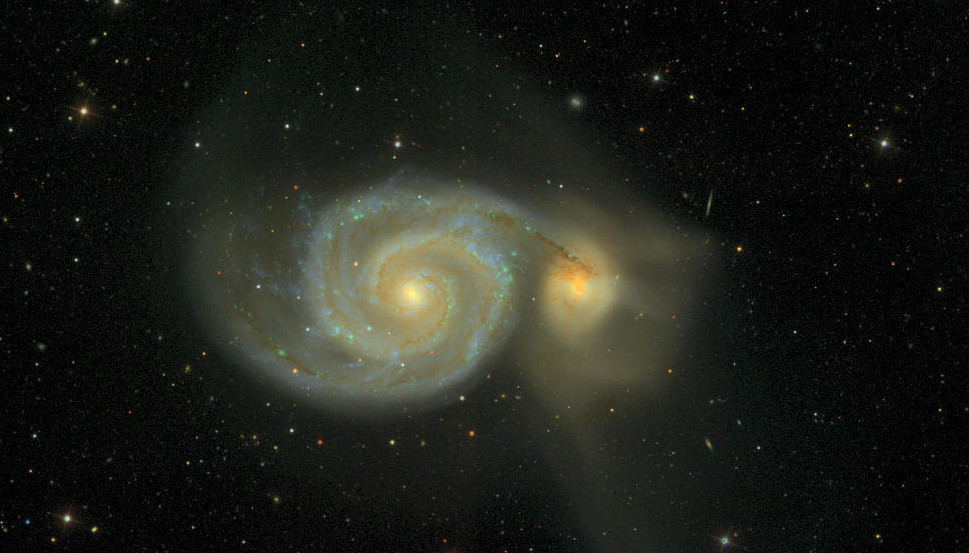
\includegraphics[width=0.8\textwidth]{M51-4x4-crop.jpg}
                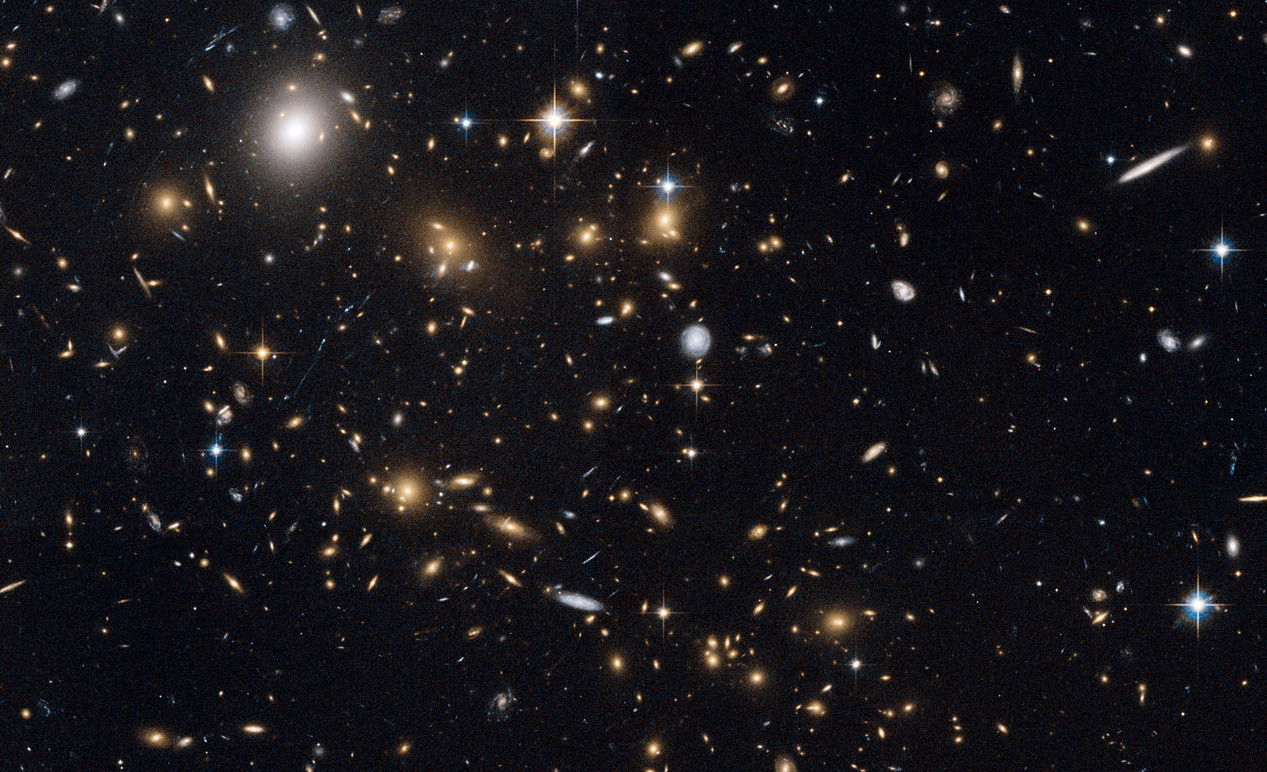
\includegraphics[width=0.8\textwidth]{macs-cluster-crop.jpg}
                \includegraphics[width=0.8\textwidth]{sdss-gals-blanton.jpg}
            \end{center}
        \end{column}
    \end{columns}
}

\frame
{
    \frametitle{Cosmology and Dark Energy}

    \setbeamerfont*{itemize/enumerate body}{size=\Large}
    \setbeamerfont*{itemize/enumerate subbody}{parent=itemize/enumerate body}
    \setbeamerfont*{itemize/enumerate subsubbody}{parent=itemize/enumerate body}

    \begin{itemize}

        \item Given initial conditions and the contents of the universe,
            we can explain much of what we see using General Relativity
            and Particle Physics

        \begin{itemize}
                
            \item Expansion history of the universe

            \item Light element abundance

            \item Cosmic microwave background

        \end{itemize}

    \item But there are a few mysteries.

    \end{itemize}
}

\frame
{
    \frametitle{Mysteries}

    \setbeamerfont*{itemize/enumerate body}{size=\Large}
    \setbeamerfont*{itemize/enumerate subbody}{parent=itemize/enumerate body}
    \setbeamerfont*{itemize/enumerate subsubbody}{parent=itemize/enumerate body}

    \begin{itemize}

        \item A few mysteries

        \begin{itemize}
                
            \item Why is the universe so homogeneous?  We know of no a priori 
                reason.  We invented {\color{gold} Inflation}.

            \item For a consistent picture we need a lot more matter than we {\it see},
                or a new theory of gravity.  We invented {\color{gold} Dark Matter}.

            \item The expansion of the universe appears to be accelerating
                rather than decelerating.  We invented {\color{gold} Dark Energy}.

        \end{itemize}

    \end{itemize}
}

\frame
{
    \frametitle{The Accelerating Universe}

    \begin{columns}
        \begin{column}{0.5\textwidth}    
            \begin{itemize}

                \item Discovered using a type of supernova that is a ``standard
                    candle'', given their apparent brightness we can determine
                    how far away it is (Riess et al. 1998, Perlmutter et al. 1999)
                        
                \item The curve of brightness vs. distance doesn't look right.

                \item Implies that the universe decelerated early on,
                    but began to accelerate later.

            \end{itemize}
        \end{column}
        \begin{column}{0.5\textwidth}    
            \begin{center}
                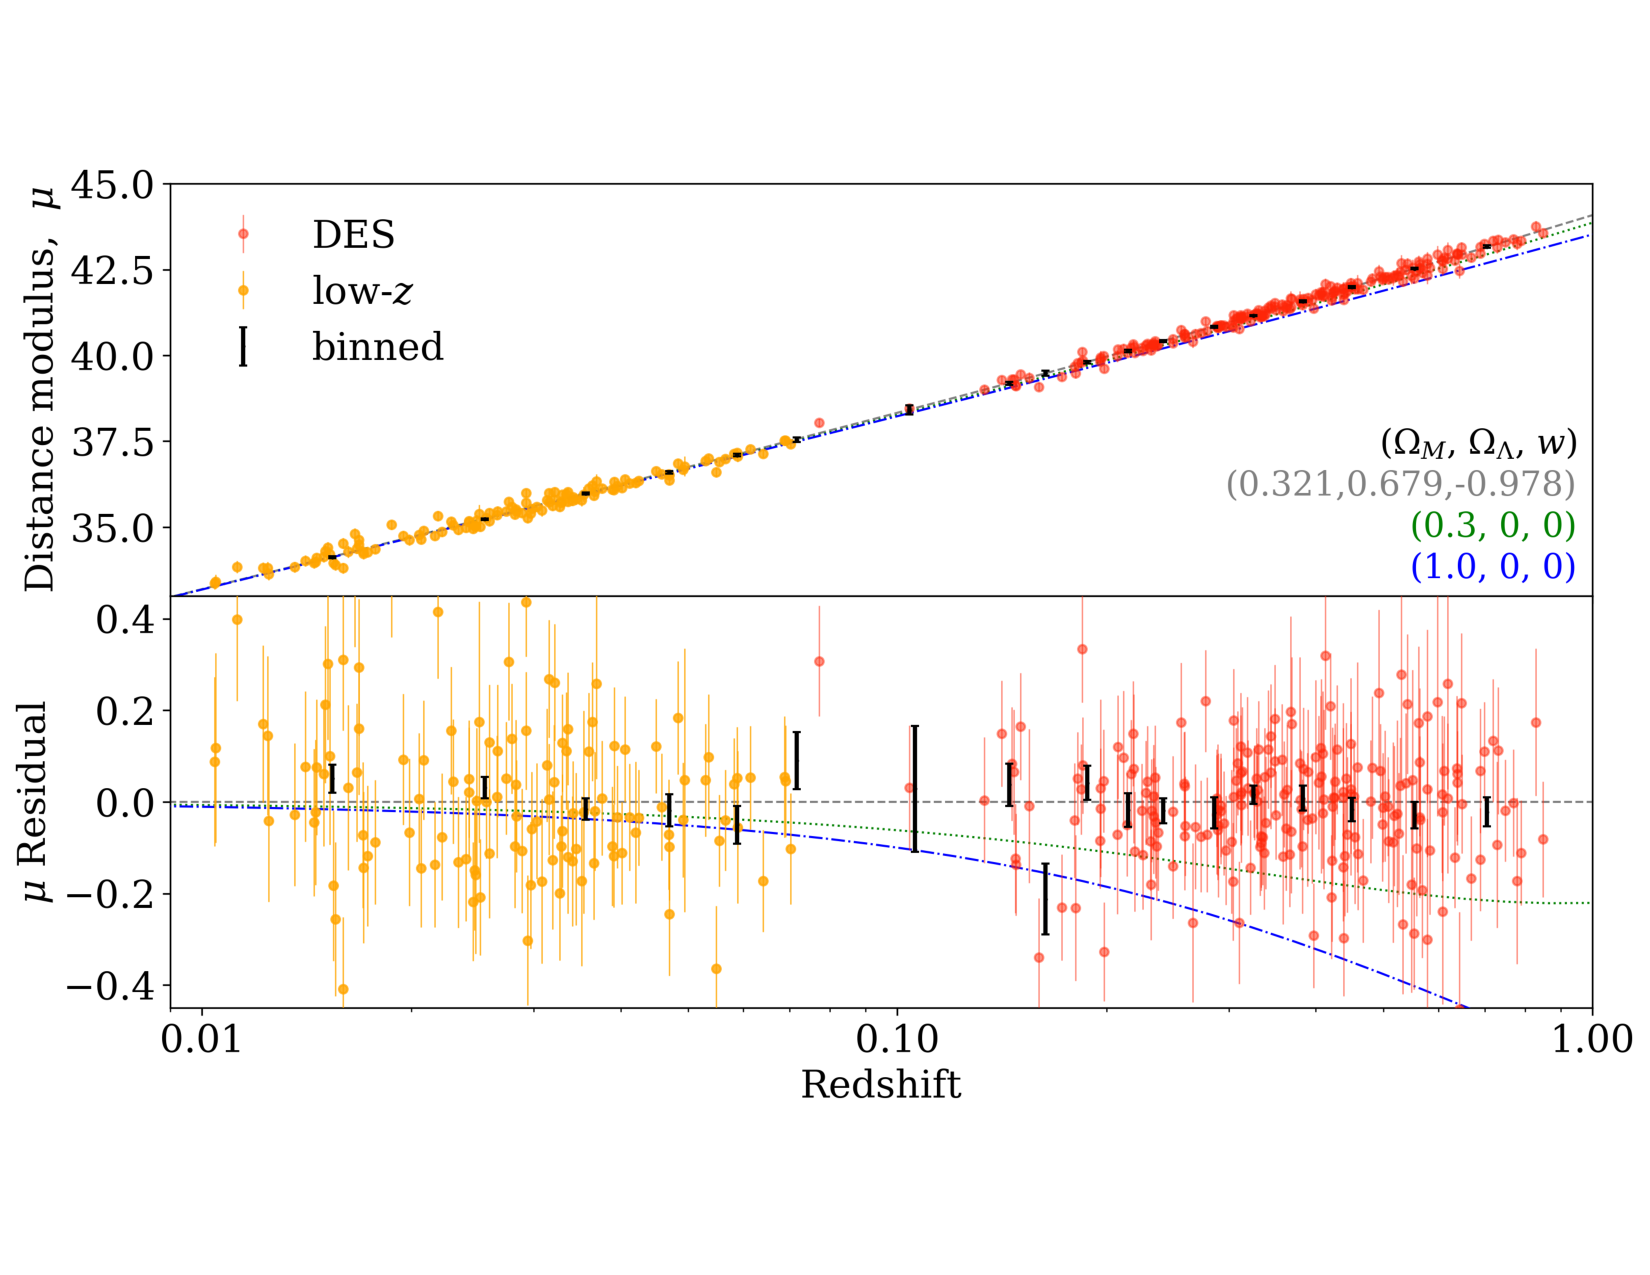
\includegraphics[width=\textwidth]{hubble_diagram_combined.pdf}
                {\tiny Dark Energy Survey, Abbott et al. 2018}
            \end{center}
        \end{column}
    \end{columns}

}

\frame
{
    \frametitle{Why is this a mystery?}

    \begin{itemize}
        \item We can use the Einstein field equations to derive the
            acceleration.
            \begin{equation}
                G_{\mu, \nu} = \frac{8 \pi G}{c^4} T_{\mu, \nu}
            \end{equation}
            Putting in a homogeneous and isotropic universe with
            density $\rho(t)$ we can
            derive the dynamics for, say, the distance $R$ between
            two distant galaxies
            \begin{equation}
                \ddot{R} = -\frac{4 \pi G c^2}{3} R(t) \rho(t)
            \end{equation}

        \item All the terms on the right hand side are positive!
    \end{itemize}
}

\frame
{
    \frametitle{What did we leave out?}

    \begin{itemize}
        \item We could include pressure {\color{gold} $p$} as well
            \begin{equation}
                \ddot{R} = -\frac{4 \pi G c^2}{3} R(t) \left[\rho(t) + \frac{3}{c^2} {\color{gold} p}\right]
            \end{equation}
            But normal matter doesn't have enough pressure, and even if it did it
            has the wrong sign:  $p = w \rho$ with $w$ positive.

    \end{itemize}
}

\frame
{
    \frametitle{What did we leave out?}

    \begin{itemize}
        \item We could include Einstein's cosmological constant fudge factor $\Lambda$:
            \begin{equation} 
                G_{\mu, \nu} + \Lambda g_{\mu, \nu} = \frac{8 \pi G}{c^4} T_{\mu, \nu}
            \end{equation}

            \begin{equation}
                \ddot{R} = -\frac{4 \pi G c^2}{3} R(t) \left[\rho(t) + \frac{3}{c^2} {\color{gold} p} - \frac{{\color{gold} \Lambda}}{3}\right]
            \end{equation}

        \item Either we need a cosmological constant {\color{gold} $\Lambda$} or we need
            some bizarre field with negative pressure {\color{gold} $p$}.

        \item If these are small compared to the matter density $\rho$ early, but becomes
            dominate late, we can explain the universe decelerating then accelerating.

    \end{itemize}
}



\frame
{
    \frametitle{Cosmology and Dark Energy}

    \setbeamerfont*{itemize/enumerate body}{size=\Large}
    \setbeamerfont*{itemize/enumerate subbody}{parent=itemize/enumerate body}
    \setbeamerfont*{itemize/enumerate subsubbody}{parent=itemize/enumerate body}

    \begin{itemize}

        \item Given initial conditions and the contents of the universe,
            we can explain much of what we see using General Relativity
            and Particle Physics

        \begin{itemize}
                
            \item Expansion history of the universe

            \item Light element abundance

            \item Cosmic microwave background

        \end{itemize}

    \item But there are a few mysteries.

    \end{itemize}
}



\frame
{

    {\Large 
        {\em Do not Bodies act upon light at a distance, and by their action bend its Rays;
        and is not this action } (caeteris paribus) {\em strongest at the least distance?}
        \newline

        \hfill - Isaac Newton (Query I, Opticks, 1704)
    }
}

\frame
{
    \frametitle{Gravitational Lensing}

    \setbeamerfont*{itemize/enumerate body}{size=\large}
    \setbeamerfont*{itemize/enumerate subbody}{parent=itemize/enumerate body}
    \setbeamerfont*{itemize/enumerate subsubbody}{parent=itemize/enumerate body}
 
    \begin{itemize}

        \item Newton's first Query, Opticks, 1704
            \begin{itemize}
                \item One can naively ``cancel'' the zero masses and predict
                    the effect
            \end{itemize}

        \item Einstein 1911
            \begin{itemize}

                \item Equivalence principle

                \item Observers in free fall experience an inertial frame.  The
                    light appears to follow straight lines: the light falls
                    with them.

            \end{itemize}

        \item Einstein 1915
            \begin{itemize}
                \item Full result from general relativity, factor of two larger
            \end{itemize}


    \end{itemize}

}


%{
%	\definecolor{mblack}{RGB}{0,0,0}
%    \setbeamertemplate{background canvas}[vertical shading][bottom=black,top=black]
	
    \frame
    {
        \frametitle{1919 Eclipse}

        %\fontsize{9}{0.8\baselineskip}
        \begin{columns}
            \begin{column}{0.5\textwidth}    
                \begin{itemize}

                    \item Einstein predicted the light from background stars would
                        be deflected as it passes near the sun.

                    \item Eddington and colleagues observed the 1919 eclipse
                        looking for the effect.

                    \item The locations of stars with known positions were
                        measured, and found to have moved

                \end{itemize}
            \end{column}
            \begin{column}{0.5\textwidth}
                \begin{center}
                    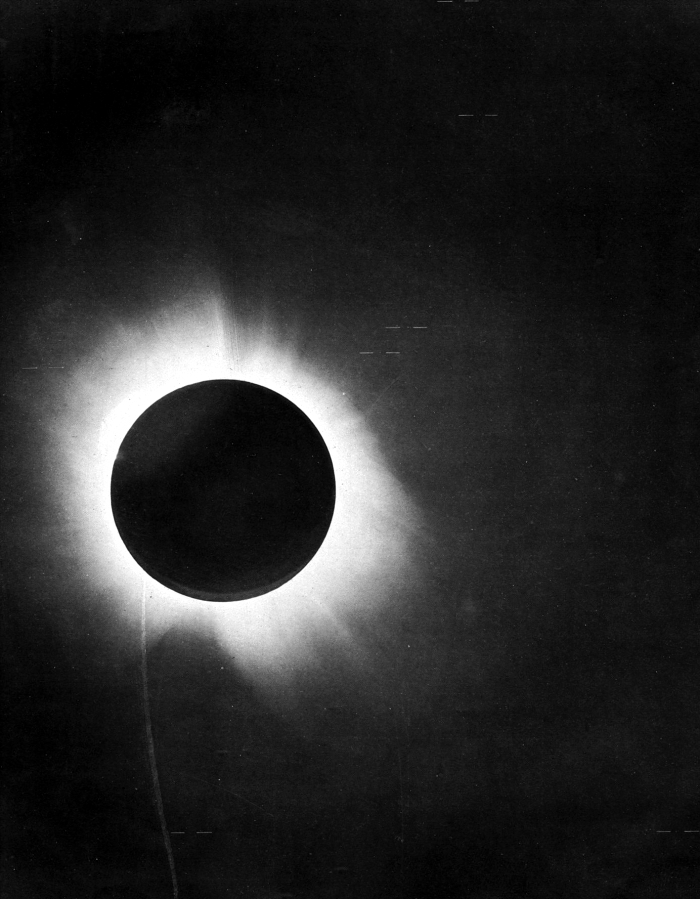
\includegraphics[width=\textwidth]{1919_eclipse_positive.jpg}
                    \newline
                    {\tiny Dyson, Eddington, Davidson 1919}
                \end{center}
            \end{column}
        \end{columns}
    }

%	\definecolor{mblack}{RGB}{50,50,50}
%    \setbeamertemplate{background canvas}[vertical shading][bottom=mgray,top=mblack]

%}

\frame
{
    \frametitle{Lensing Geometry}

    \begin{center}
        
\includegraphics[scale=0.4]{lens_geometry_invert.pdf}
        \newline
        For a point mass lens, the deflection depends on impact
        prameter and mass as
        \newline
        {\huge {\color{gold} $\alpha \propto \frac{M}{b}$ }}
    \end{center}
}



\frame
{
    \frametitle{Twin Quasar 0957+0561}

    %\fontsize{9}{0.8\baselineskip}
    \begin{columns}
        \begin{column}{0.5\textwidth}    
            \begin{itemize}

                \item Two quasars discovered in 1979 (Walsh, Carswell, Weyman)

                \item Extremely close together, nearly identical spectrum and redshift

                \item Time variations in image A appear in image B also, but 14 months later.

                \item Two images of the same object!
                    
            \end{itemize}
        \end{column}
        \begin{column}{0.5\textwidth}
            \begin{center}
                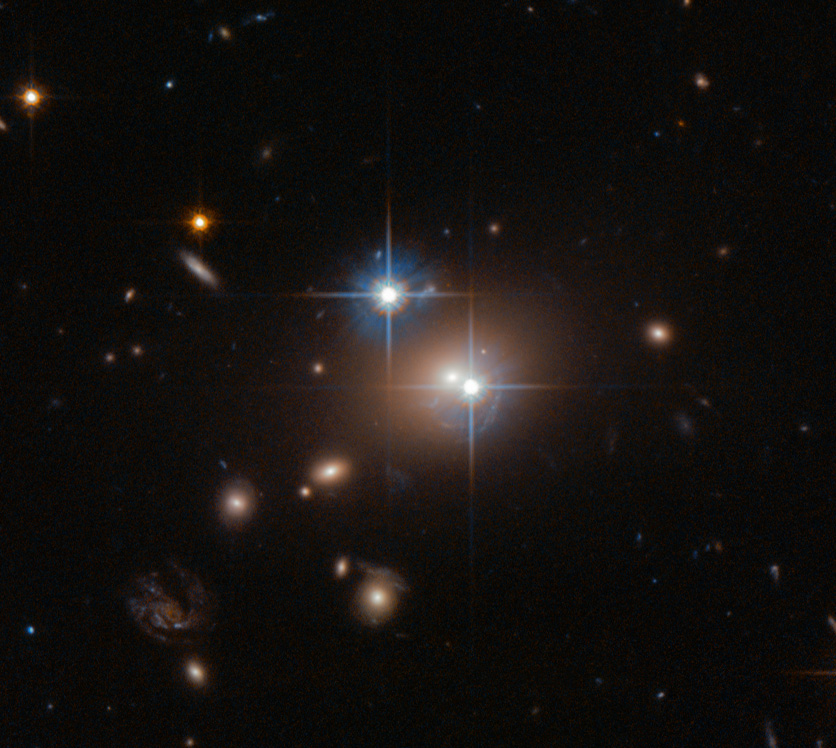
\includegraphics[width=\textwidth]{QSO_B0957+0561-crop.jpg}
                \newline
                {\tiny ESA/Hubble \& NASA}
            \end{center}
        \end{column}
    \end{columns}
}

\frame
{
    \frametitle{Twin Quasars: {\color{gold} Can infer $\alpha$}}

    \begin{center}
        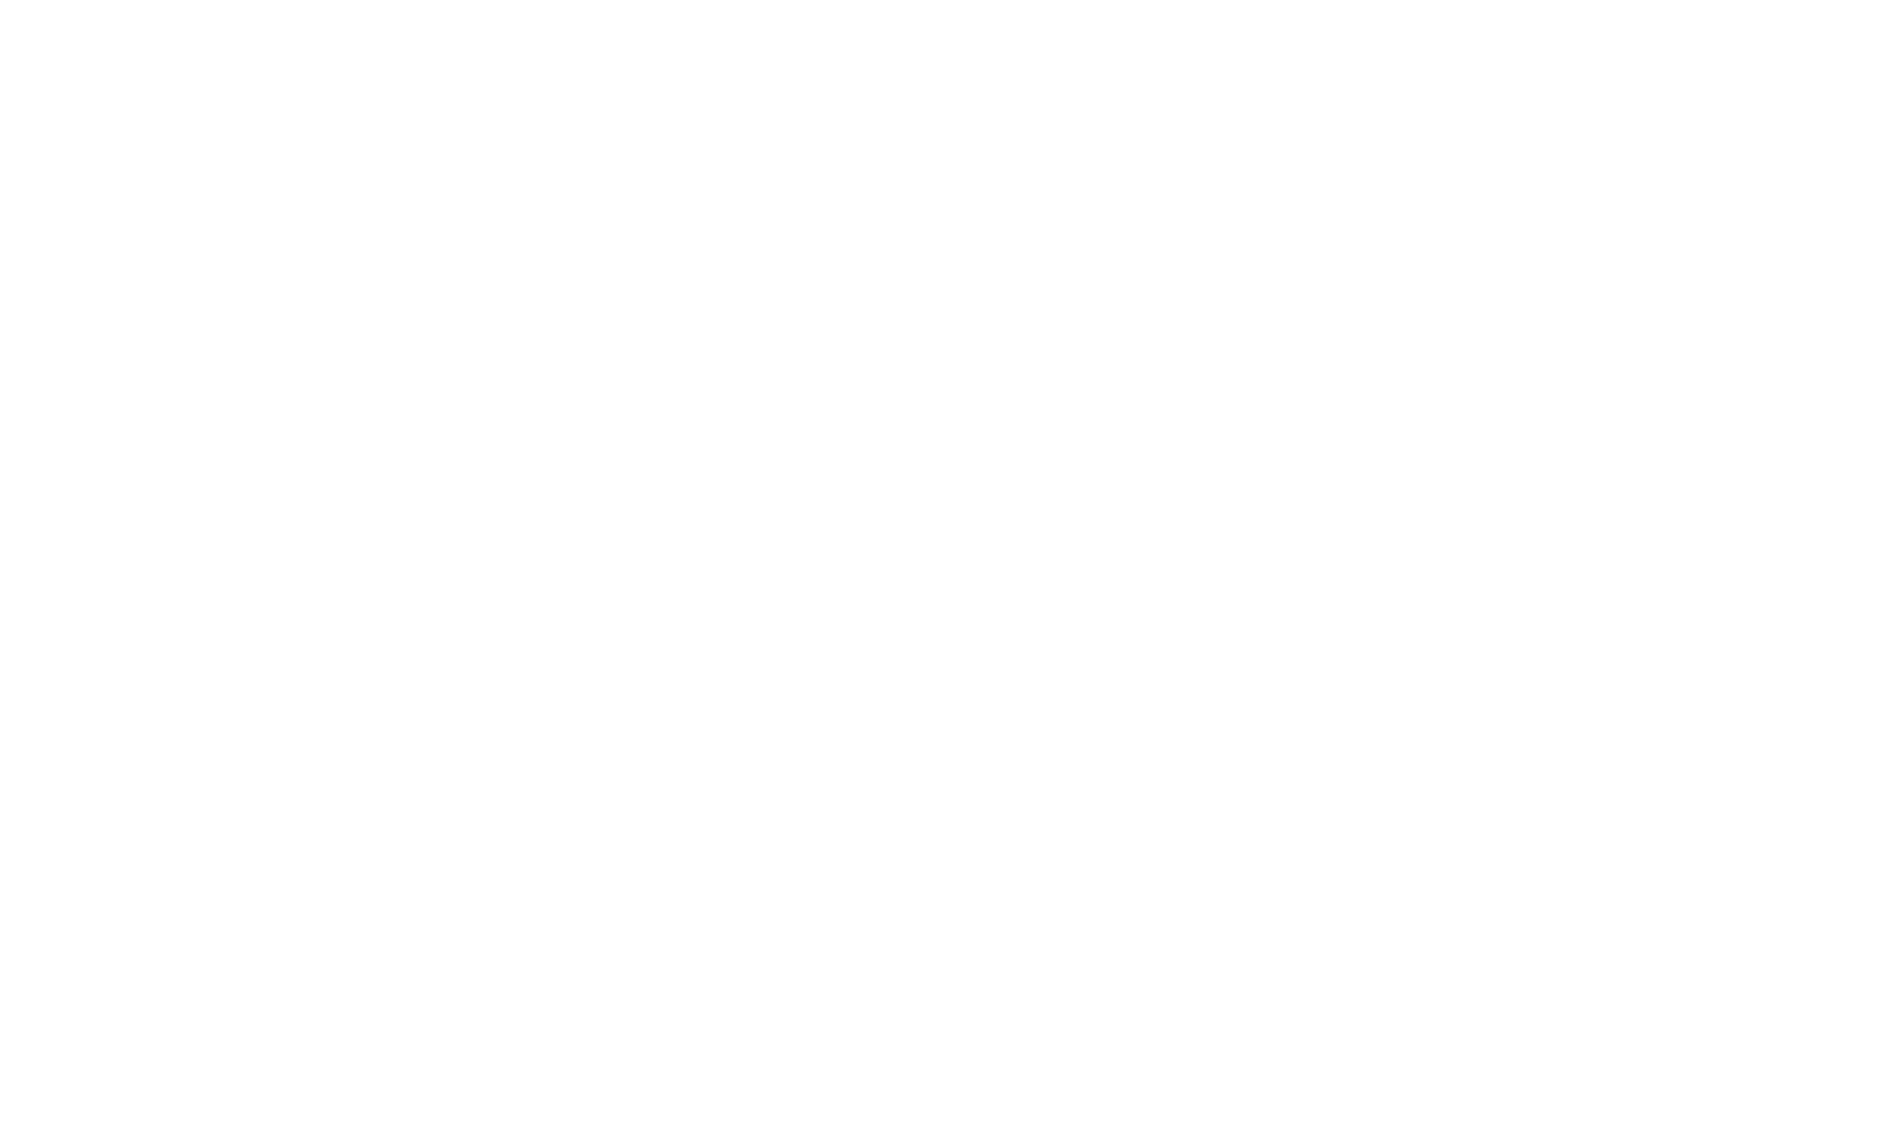
\includegraphics[width=\textwidth]{glensing.png}
    \end{center}
        %\newline
        \hfill  {\tiny User Krishnavedala, {\em wikipedia} }
}


{
	\definecolor{mblack}{RGB}{0,0,0}
    \setbeamertemplate{background canvas}[vertical shading][bottom=black,top=black]
	
    \frame
    {
        \frametitle{Einstein Ring: The ``Horseshoe''}

        \begin{center}
            \includegraphics[height=0.7\textheight]{A_Horseshoe_Einstein_Ring_from_Hubble.JPG}

            {\tiny \hfill ESA/Hubble \& NASA}
        \end{center}
    }

	\definecolor{mblack}{RGB}{50,50,50}
    \setbeamertemplate{background canvas}[vertical shading][bottom=mgray,top=mblack]

}


\begin{comment}
    {
        \definecolor{mblack}{RGB}{0,0,0}
        \setbeamertemplate{background canvas}[vertical shading][bottom=black,top=black]

        \frame
        {
            \frametitle{Lensing by Galaxy Clusters: Abell 1689}

            \begin{center}
                \includegraphics[height=0.8\textheight]{abell1689_hubble_1280.jpg}

                {\tiny \hfill NASA, ESA, STScI/AURA, J. Blakeslee, H. Ford}
            \end{center}
        }

        \definecolor{mblack}{RGB}{50,50,50}
        \setbeamertemplate{background canvas}[vertical shading][bottom=mgray,top=mblack]

    }

    {
        \definecolor{mblack}{RGB}{0,0,0}
        \setbeamertemplate{background canvas}[vertical shading][bottom=black,top=black]

        \frame
        {
            \begin{center}
                \includegraphics[height=0.9\textheight]{abell1689-details.pdf}
            \end{center}
        }

        \definecolor{mblack}{RGB}{50,50,50}
        \setbeamertemplate{background canvas}[vertical shading][bottom=mgray,top=mblack]

    }
\end{comment}


{
	\definecolor{mblack}{RGB}{0,0,0}
    \setbeamertemplate{background canvas}[vertical shading][bottom=black,top=black]
	
    \frame
    {
        \frametitle{Shear Illustration}
        \begin{center}
            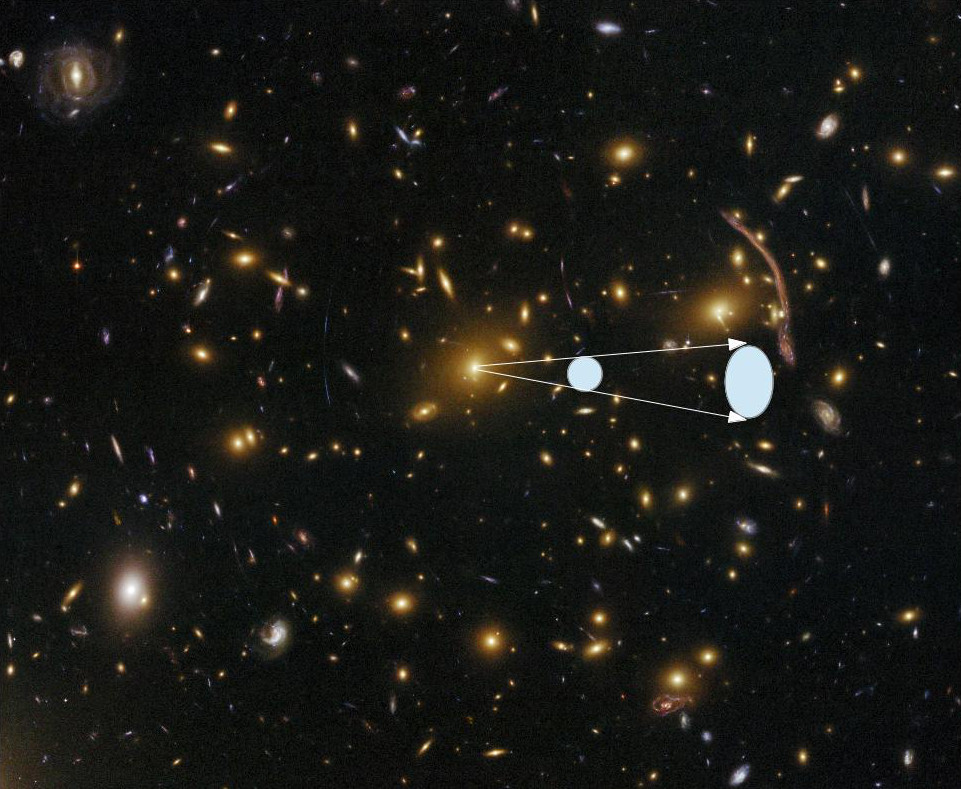
\includegraphics[height=0.8\textheight]{shear-illustration-nowhite.jpg}
        \end{center}
    }

	\definecolor{mblack}{RGB}{50,50,50}
    \setbeamertemplate{background canvas}[vertical shading][bottom=mgray,top=mblack]

}


	
\frame
{
    \frametitle{Shear Illustration}

    \begin{columns}
        \begin{column}{0.5\textwidth}    
            \begin{itemize}

                \item The shape of extended background sources is changed.

                \item The differential deflections across the surface
                    of the background image produces a shear.

                \item For strong lensing a round source becomes a ``banana''

                \item For {\color{gold} weak lensing} a round source becomes slightly elliptical

            \end{itemize}
        \end{column}
        \begin{column}{0.5\textwidth}
            \begin{center}
                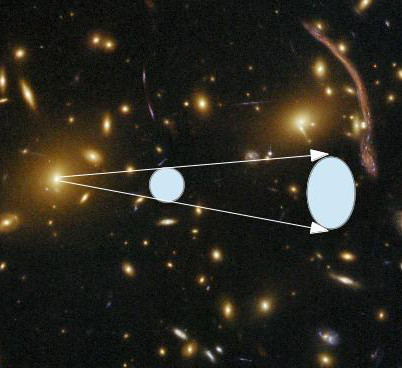
\includegraphics[width=\textwidth]{shear-illustration-crop2.jpg}
                \newline
                {\small Tangential Shear}
            \end{center}
        \end{column}
    \end{columns}
}

\frame
{
    \frametitle{Weak Lensing}

    \begin{columns}

        \begin{column}{0.5\textwidth}
            \begin{center}
                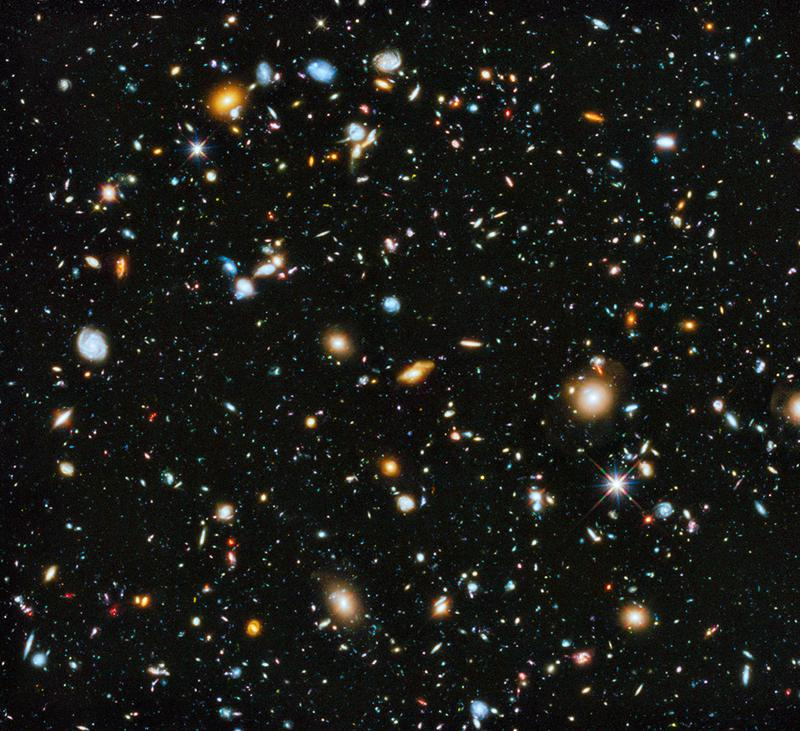
\includegraphics[width=\textwidth]{hubble-ultra-deep-scaled.jpg}
                \newline
                {\tiny  NASA/ESA, Teplitz et al.}
            \end{center}
        \end{column}

        \begin{column}{0.5\textwidth}    
            \begin{itemize}

                \item Strong lensing requires special, fortuitous alignments.
                    Not that useful as a general tool

                \item But everything is lensed slightly, and the {\color{gold} tangential shear}
                    pattern is imprinted all over the sky.

                \item Taking a statistical approach, we can study the mass
                    distribution around any set of objects.

            \end{itemize}
        \end{column}

    \end{columns}
}


{
	\definecolor{mblack}{RGB}{0,0,0}
    \setbeamertemplate{background canvas}[vertical shading][bottom=black,top=black]
	
    \frame
    {
        \frametitle{Weak Lensing: Tangential Shear}
            
            \begin{minipage}{\linewidth}
                \begin{center}
                    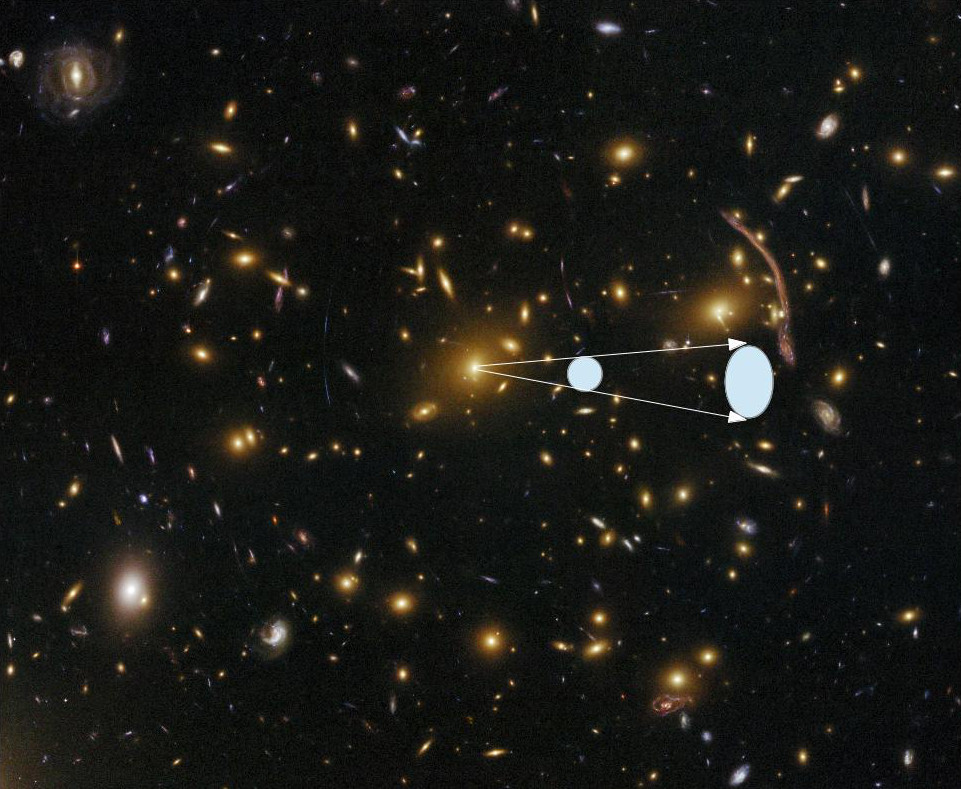
\includegraphics[height=0.6\textheight]{shear-illustration-nowhite.jpg}
                \end{center}
            \end{minipage}

            \begin{minipage}{\linewidth}
                \begin{center}
                    {\color{gold}
                        {\huge
                            $\overline{e}_{T}(R) \propto \overline{\Sigma}(<R) - \overline{\Sigma}(R)$
                        }
                    }
                \end{center}
            \end{minipage}

    }


	\definecolor{mblack}{RGB}{50,50,50}
    \setbeamertemplate{background canvas}[vertical shading][bottom=mgray,top=mblack]

}


\frame
{

    {\Huge Dark Matter}

}



\frame
{
    \frametitle{Dark Matter}

    \begin{columns}

        \begin{column}{0.5\textwidth}
            \begin{center}
                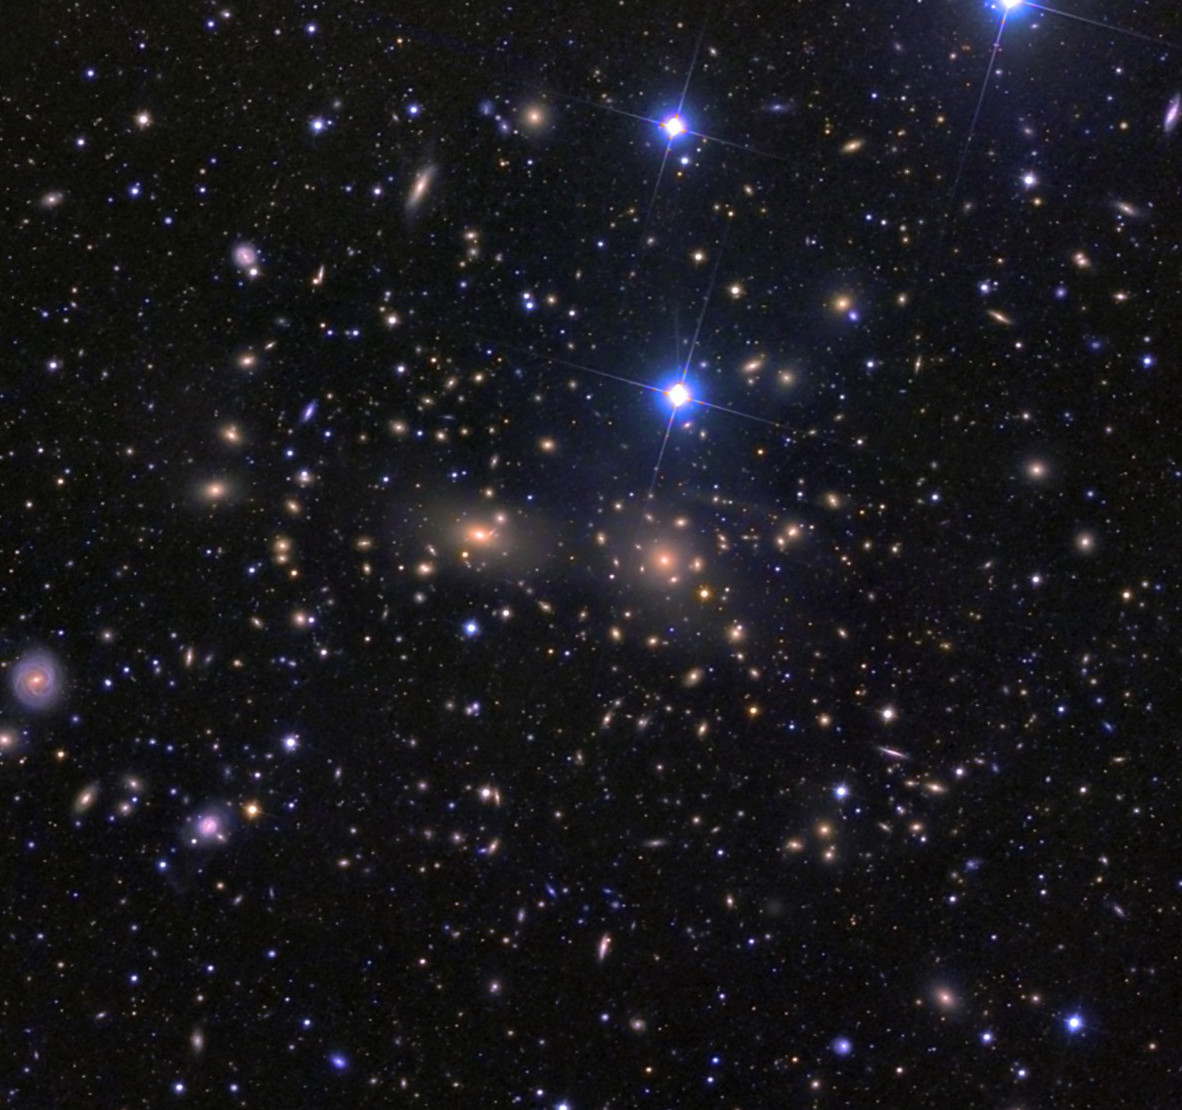
\includegraphics[width=\textwidth]{comacluster_rowe_big_crop.jpg}
                \newline
                {\tiny Dean Rowe}
            \end{center}
        \end{column}



        \begin{column}{0.5\textwidth}    
            \begin{itemize}

                \item Fritz Zwicky 1933

                \item He found the galaxies in the Coma cluster were moving far
                    too fast.

                \item Assuming equilibrium (good to factor of two) he calculated
                    the binding mass is $\sim$ 100 times the mass in stars

            \end{itemize}
        \end{column}

    \end{columns}
}

\frame
{

    {\Large 
        {\em The observation of such gravitational lens effects promises to furnish us with
        the simplest and most accurate determination of nebular masses.}
        \newline

        \hfill - Fritz Zwicky, 1937
    }
}


\frame
{
    \frametitle{Dark Matter: Galaxy Rotation Curves}

    \begin{columns}
        \begin{column}{0.5\textwidth}    
            \begin{itemize}

                \item Rubin studied the rotation curves of galaxies in the 70s

                \item The light density falls exponentially with radius.

                \item The mass density implied by the velocities falls like a power law

                \item Extrapolation seemed to imply the mass continued well
                    beyond the region of visible stars

            \end{itemize}
        \end{column}
        \begin{column}{0.5\textwidth}
            \begin{center}
                %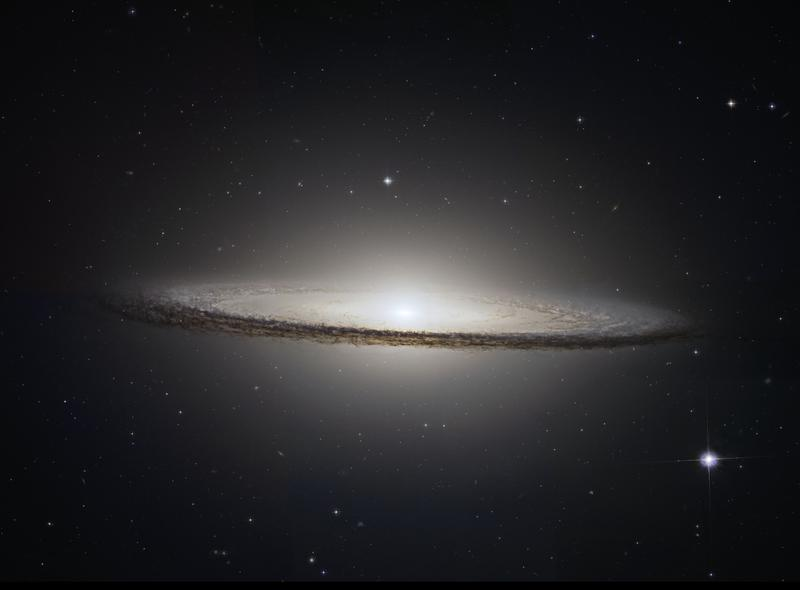
\includegraphics[width=0.8\textwidth]{m104-2013-03-01-HLA-5238-HLA-crop-scaled.jpg}
                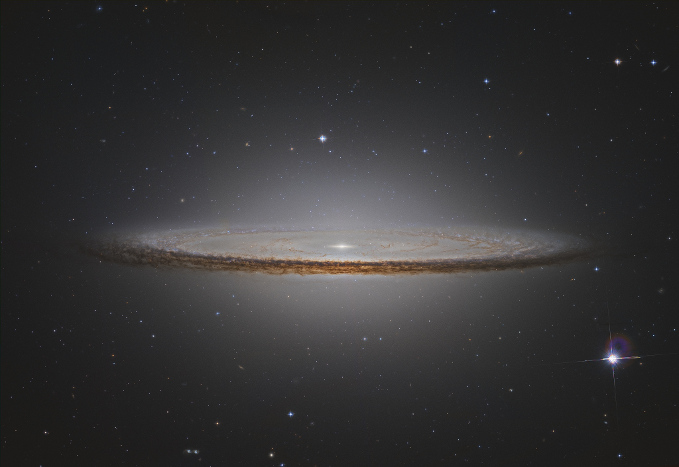
\includegraphics[width=0.8\textwidth]{M104b_peris2048_scale_small.jpg}
                \newline
                \hfill {\tiny NASA/ESA/V. Peris}

                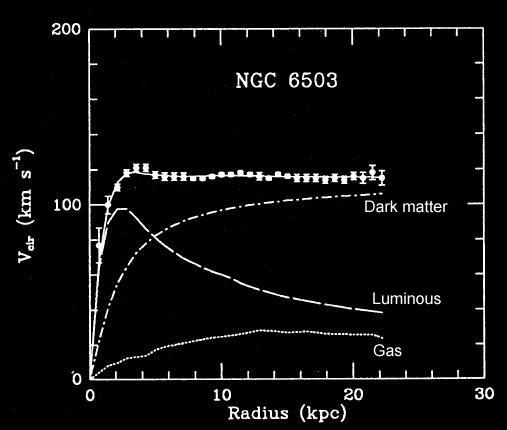
\includegraphics[width=0.8\textwidth]{ngc-6503-rotation-curve.jpg}
                \newline
                {\tiny Begeman, Broels and Sanders (1991)}
            \end{center}
        \end{column}
    \end{columns}
}

\frame
{
    \frametitle{Cold Dark Matter (CDM)}

    \setbeamerfont*{itemize/enumerate body}{size=\Large}
    \setbeamerfont*{itemize/enumerate subbody}{parent=itemize/enumerate body}
    \setbeamerfont*{itemize/enumerate subsubbody}{parent=itemize/enumerate body}

    \begin{itemize}

        \item Some form of matter that does not significantly emit or absorb light

        \item Cold:  $v \ll c$

        \item Favored idea is an elementary particle, weakly interacting

        \item So far CDM successfully explains most observations, and has been
            predictive

    \end{itemize}


}

\frame
{
    \frametitle{Early Successes of CDM}

    \setbeamerfont*{itemize/enumerate body}{size=\Large}
    \setbeamerfont*{itemize/enumerate subbody}{parent=itemize/enumerate body}
    \setbeamerfont*{itemize/enumerate subsubbody}{parent=itemize/enumerate body}
 
    \begin{itemize}

        \item Explains rotation curves of galaxies

        \item Explains the dynamics of galaxy clusters

        \item Explains the large scale distribution of galaxies: without it we
          would predict a wildly different universe

        \item Essential component needed to explain the cosmic microwave
          background

    \end{itemize}

}

\frame
{
    \frametitle{Predictions of CDM}

    \setbeamerfont*{itemize/enumerate body}{size=\Large}
    \setbeamerfont*{itemize/enumerate subbody}{parent=itemize/enumerate body}
    \setbeamerfont*{itemize/enumerate subsubbody}{parent=itemize/enumerate body}
 
    \begin{itemize}

        \item  ``Universal'' radial profile of gravitationally bound dark matter
            structures, ``halos'' (NFW, simulations)
            \begin{itemize}
                \item Running power law with one free parameter for shape
                \item Mass extends orders of magnitude farther beyond visible portion of galaxy,
                    merges with neighbors
            \end{itemize}


        \item  Dark matter should be distributed smoothly throughout the
            universe
            \begin{itemize}
                \item Unlike dissipative baryons that collapse to more compact objects
            \end{itemize}

    \end{itemize}

}

\frame
{
    \frametitle{Predictions of CDM}

    \fontsize{9}{0.8\baselineskip}
    \begin{columns}

        \begin{column}{0.5\textwidth}
            \begin{center}
                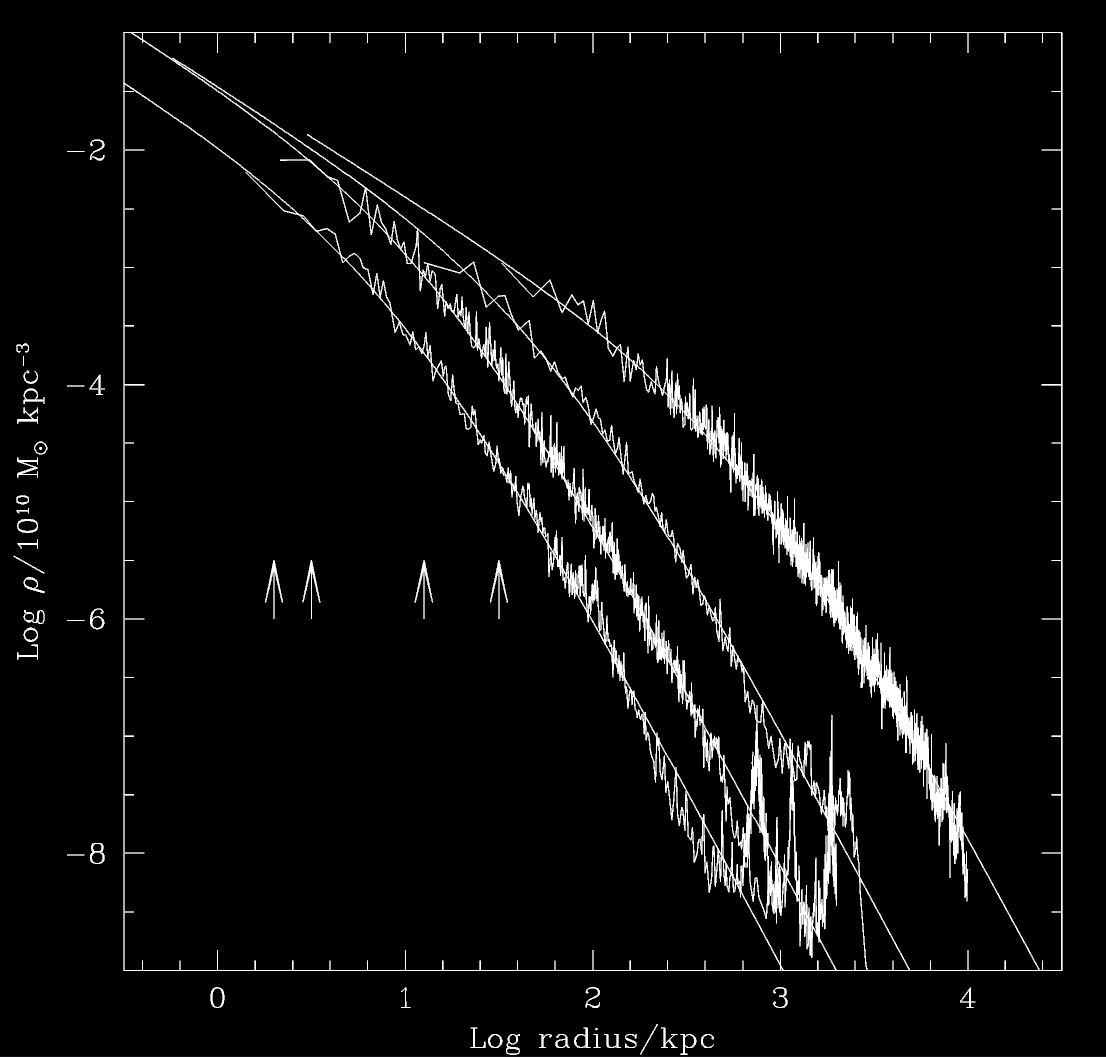
\includegraphics[width=\textwidth]{nfw.png}
                \newline
                {\tiny Navarro, Frenk, White 1996}
            \end{center}
        \end{column}

        \begin{column}{0.5\textwidth}    
            \begin{itemize}

                \item  ``Universal'' radial profile of gravitationally bound dark matter
                    structures, ``halos'' {\color{gold} (NFW)}

                    %\begin{itemize}
                        \item Running power law with one free parameter for shape

                        \item Mass extends orders of magnitude farther than visible portion of galaxy,
                            merges with neighbors
                    %\end{itemize}

                \item  Dark matter distributed smoothly throughout the
                    universe, unlike dissipative baryons clumped in galaxies.

                {\color{gold} {\tiny 1pc = 3.2 ly}}

            \end{itemize}
        \end{column}

    \end{columns}
}




\frame
{
    \frametitle{Limits of dynamical approaches}

    \begin{itemize}

        \item visible tracers are required
        \item cannot trace out the orbits, the timescales are too long
        \item assumptions must be made about the dynamical state of the system
        \item limits the scale over which it this can be used

    \end{itemize}

    %\begin{minipage}{\paperwidth}
    %    \centering
        %\begin{center}
            %{\small Scale 10 kpc}
            %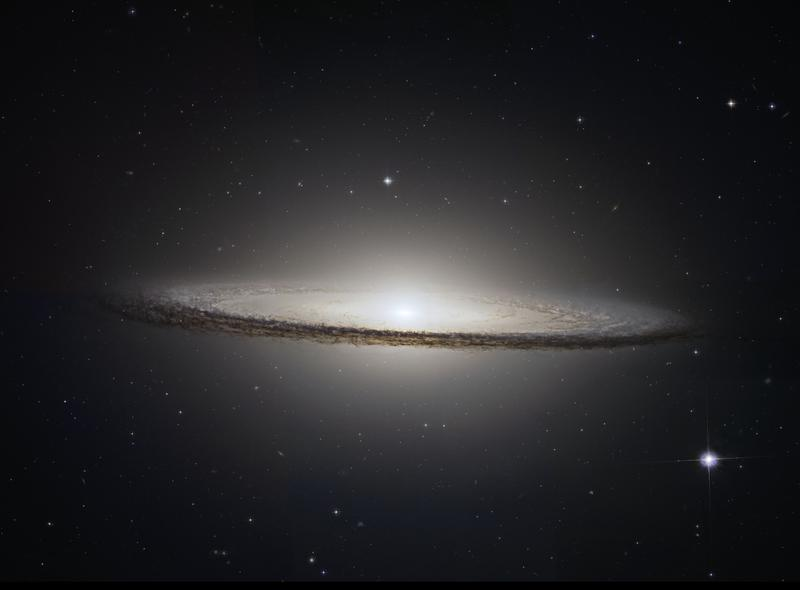
\includegraphics[width=\textwidth]{m104-2013-03-01-HLA-5238-HLA-crop-scaled.jpg}
    \centerline{Scale 10 kpc}
    \centerline{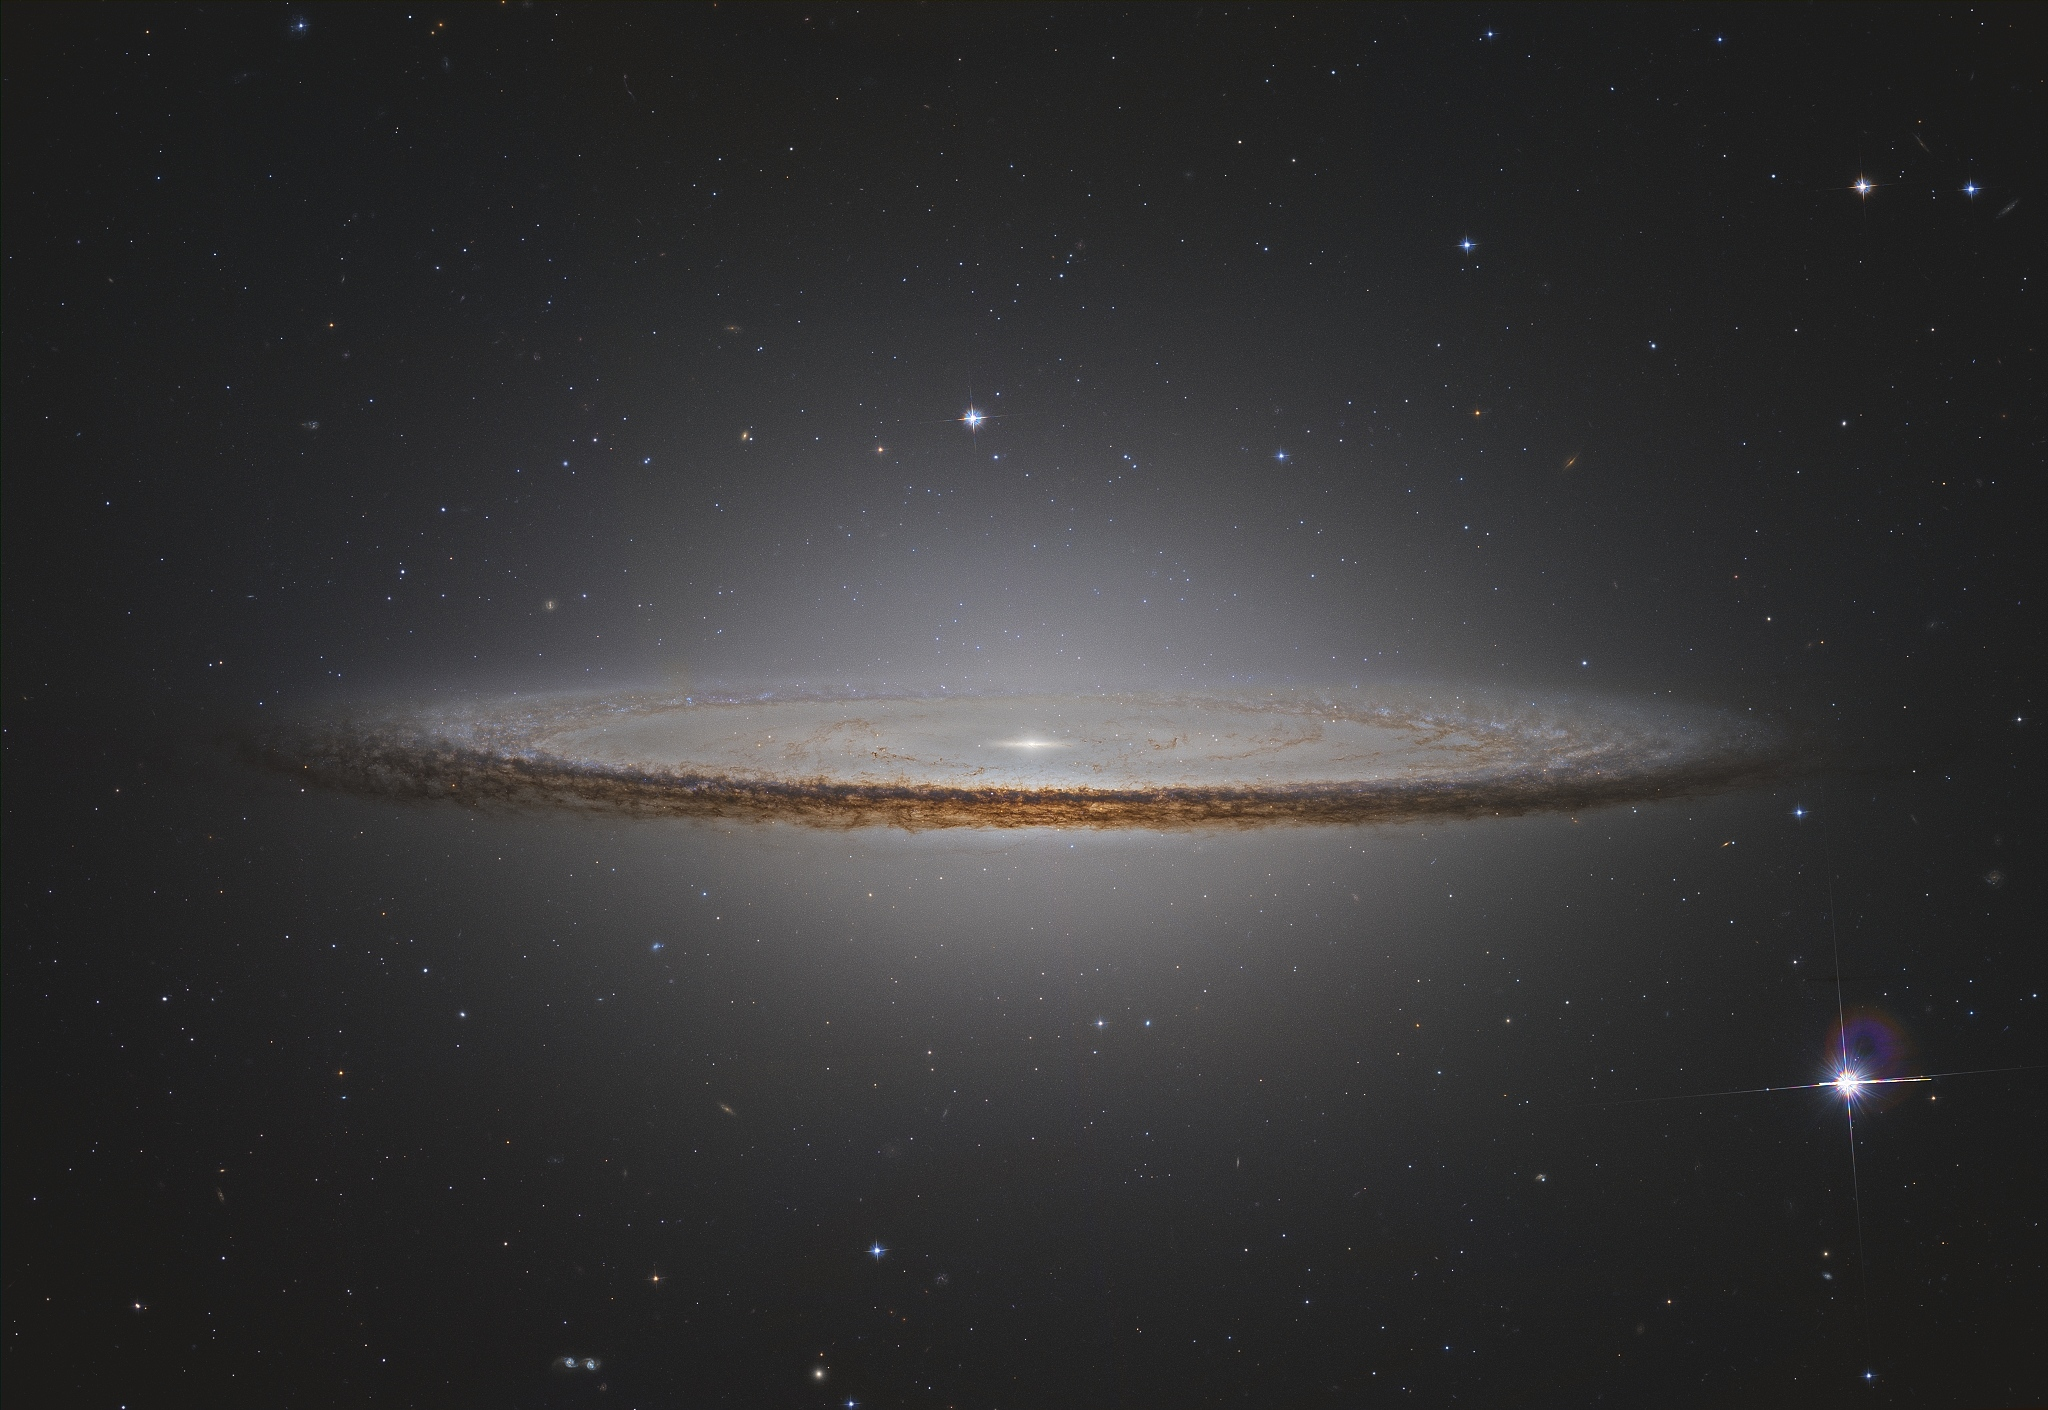
\includegraphics[trim=0 400 0 500,clip,width=\paperwidth]{M104b_peris2048.jpg}}
            \hfill {\tiny NASA/ESA/V. Peris}
        %\end{center}
    %\end{minipage}
}


\frame
{
    \frametitle{Weak Lensing is a Better Option}

    \begin{columns}
        \begin{column}{0.5\textwidth}    
            \begin{itemize}

                \item The weak effect can be observed anywhere
                \item The distribution of matter can be studied on a large range of scales
                \begin{itemize}
                    \item galaxies, galaxy clusters, bound objects
                    \item structure on the largest scales in the universe
                \end{itemize}

            \end{itemize}
        \end{column}
        \begin{column}{0.5\textwidth}
            \begin{center}
                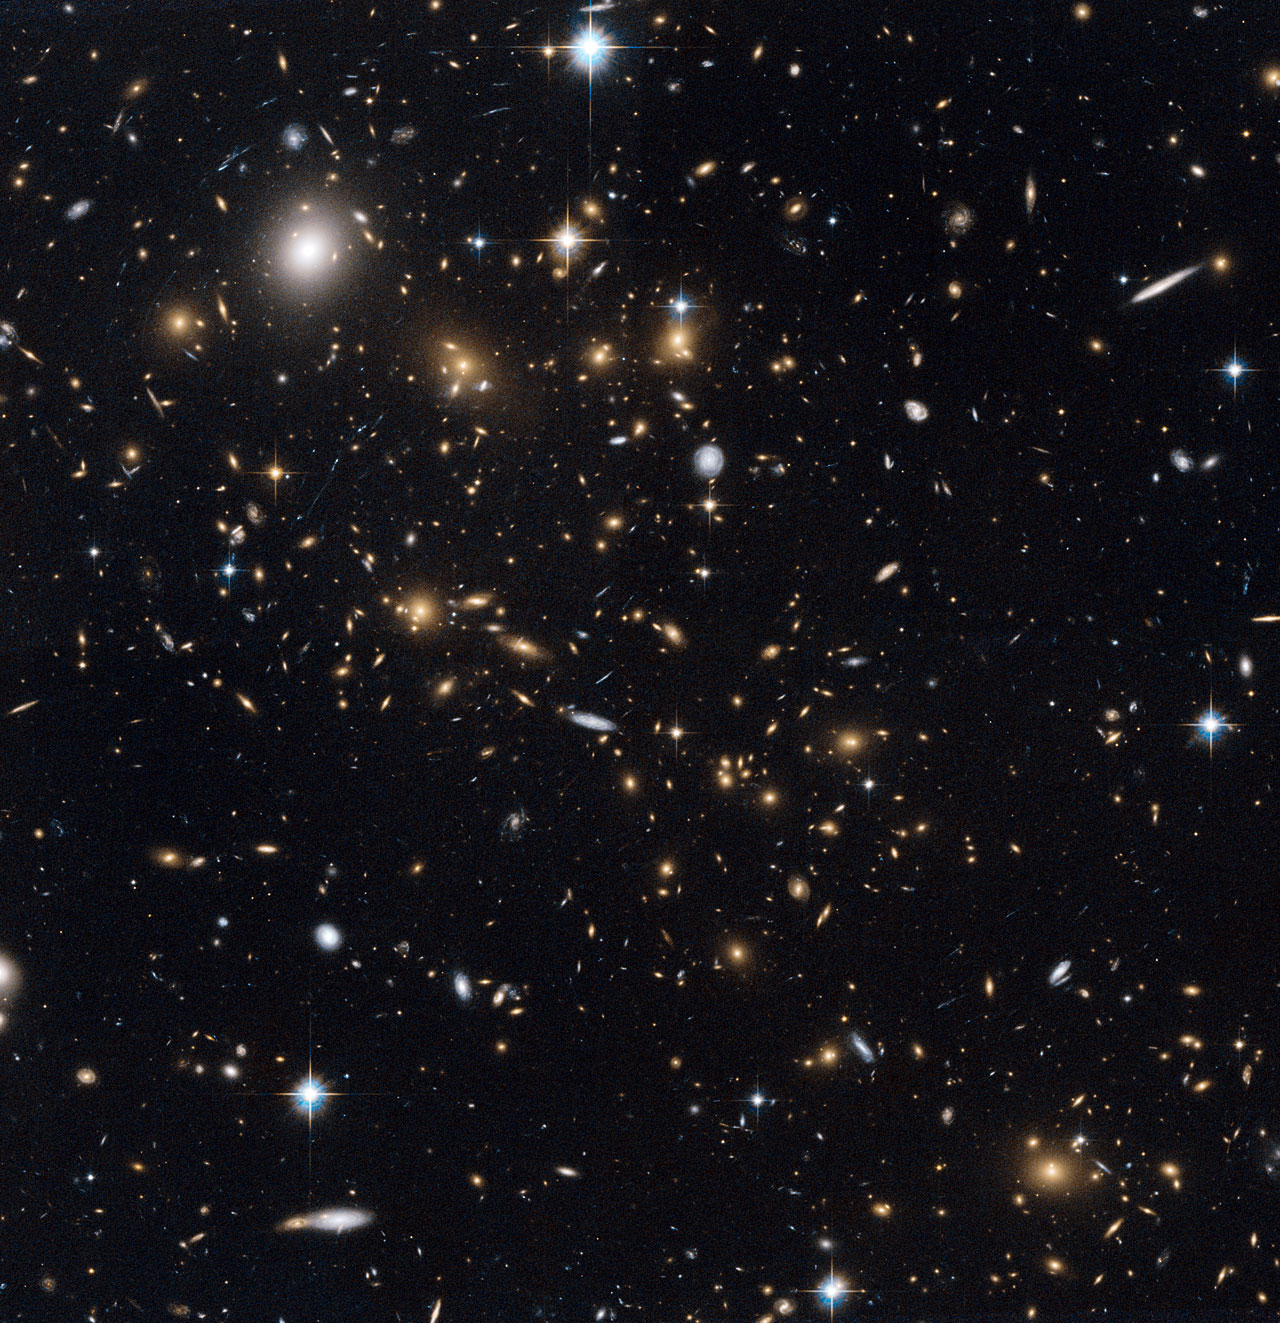
\includegraphics[width=\textwidth]{macs-cluster.jpg}
                \newline
                {\tiny NASA/ESA}
            \end{center}
        \end{column}
    \end{columns}
}


\frame
{
    \frametitle{Weak Lensing Limitations}

    \setbeamerfont*{itemize/enumerate body}{size=\Large}
    \setbeamerfont*{itemize/enumerate subbody}{parent=itemize/enumerate body}
    \setbeamerfont*{itemize/enumerate subsubbody}{parent=itemize/enumerate body}
 
    %\begin{columns}
    %    \begin{column}{0.5\textwidth}    
            \begin{itemize}

                \item The effect is very weak, percent level change in
                    ellipticity

                \item Statistical approach is required: average signal from
                    many lenses and many background sources

                \item But these are unimportant limitations. The theory doesn't
                    predict anything about individual objects anyway: these are
                    messy systems with a complicated history

            \end{itemize}
    %    \end{column}

    %    \begin{column}{0.5\textwidth}
    %        \begin{center}
    %            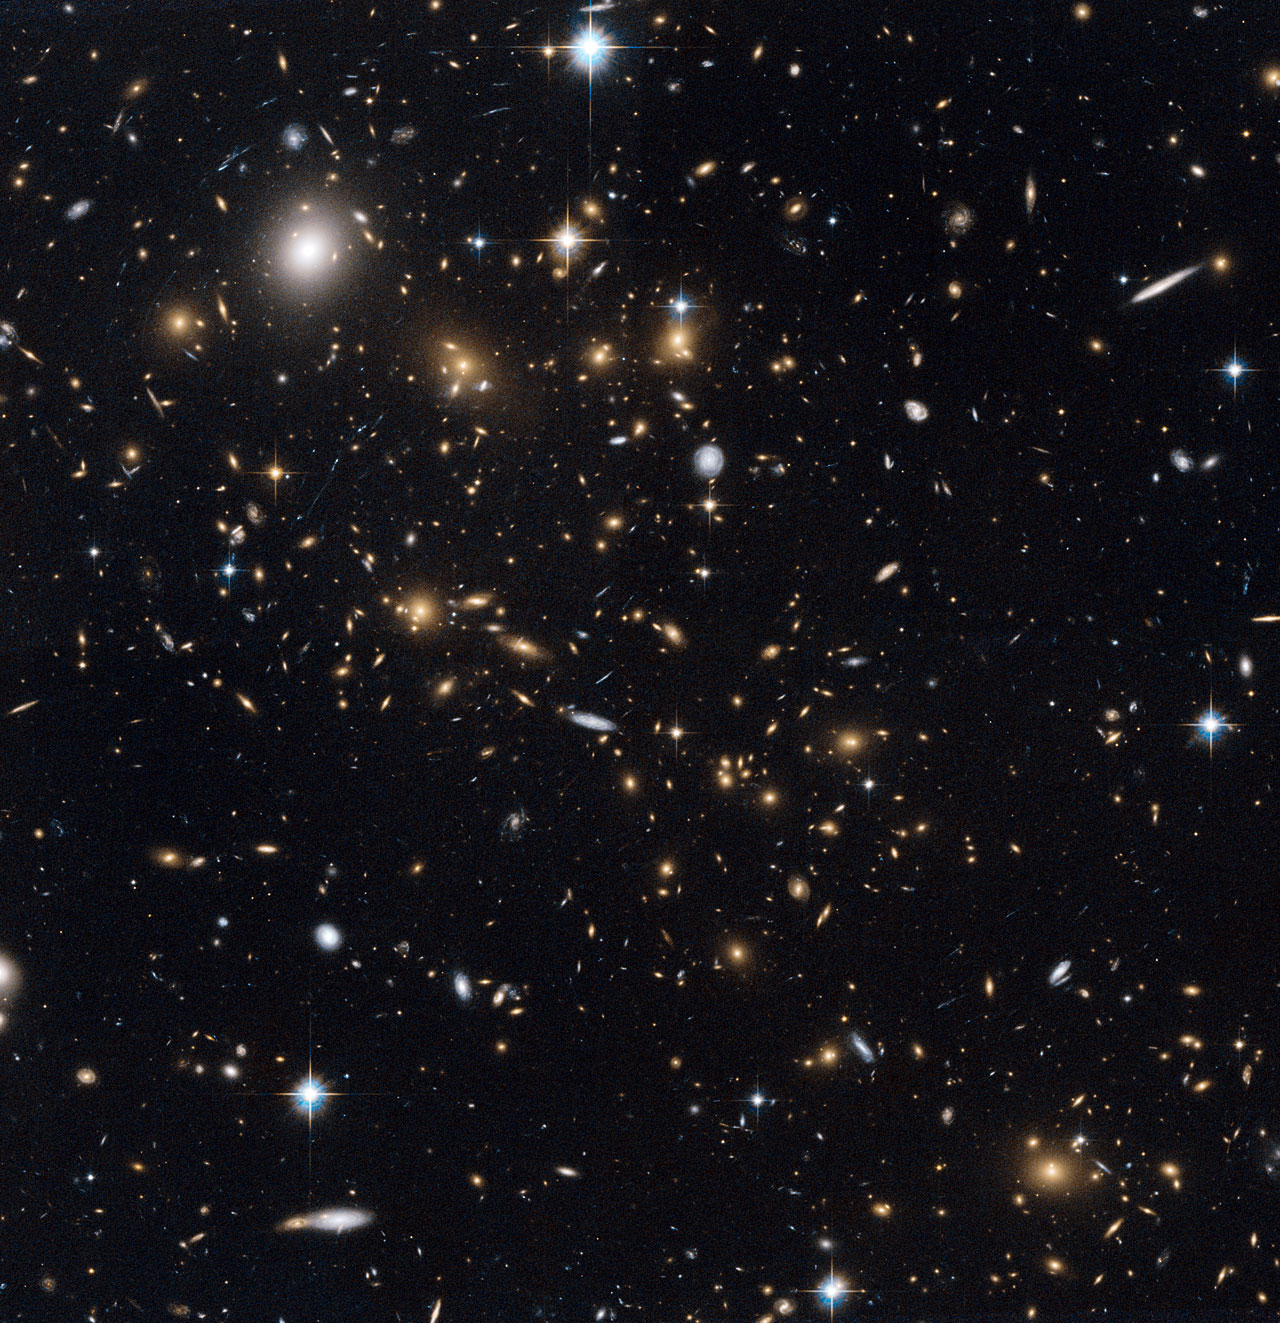
\includegraphics[width=\textwidth]{macs-cluster.jpg}
    %            \newline
    %            {\tiny NASA/ESA}
    %        \end{center}
    %    \end{column}

    %\end{columns}
}


\frame
{
    \frametitle{Weak Lensing: The Program}

    \begin{columns}
        \begin{column}{0.5\textwidth}    
            \begin{enumerate}

                \item Identify lenses, such as galaxies or cluster of galaxies

                \item Identify background sources and measure their
                    ellipticities {\color{gold}(that's the hard part!)}


                \item Average the ellipticities of background galaxies

                \item Average over lots of lenses

                \item Infer the mean radial distribution of mass

            \end{enumerate}
        \end{column}
        \begin{column}{0.5\textwidth}
            \begin{center}
                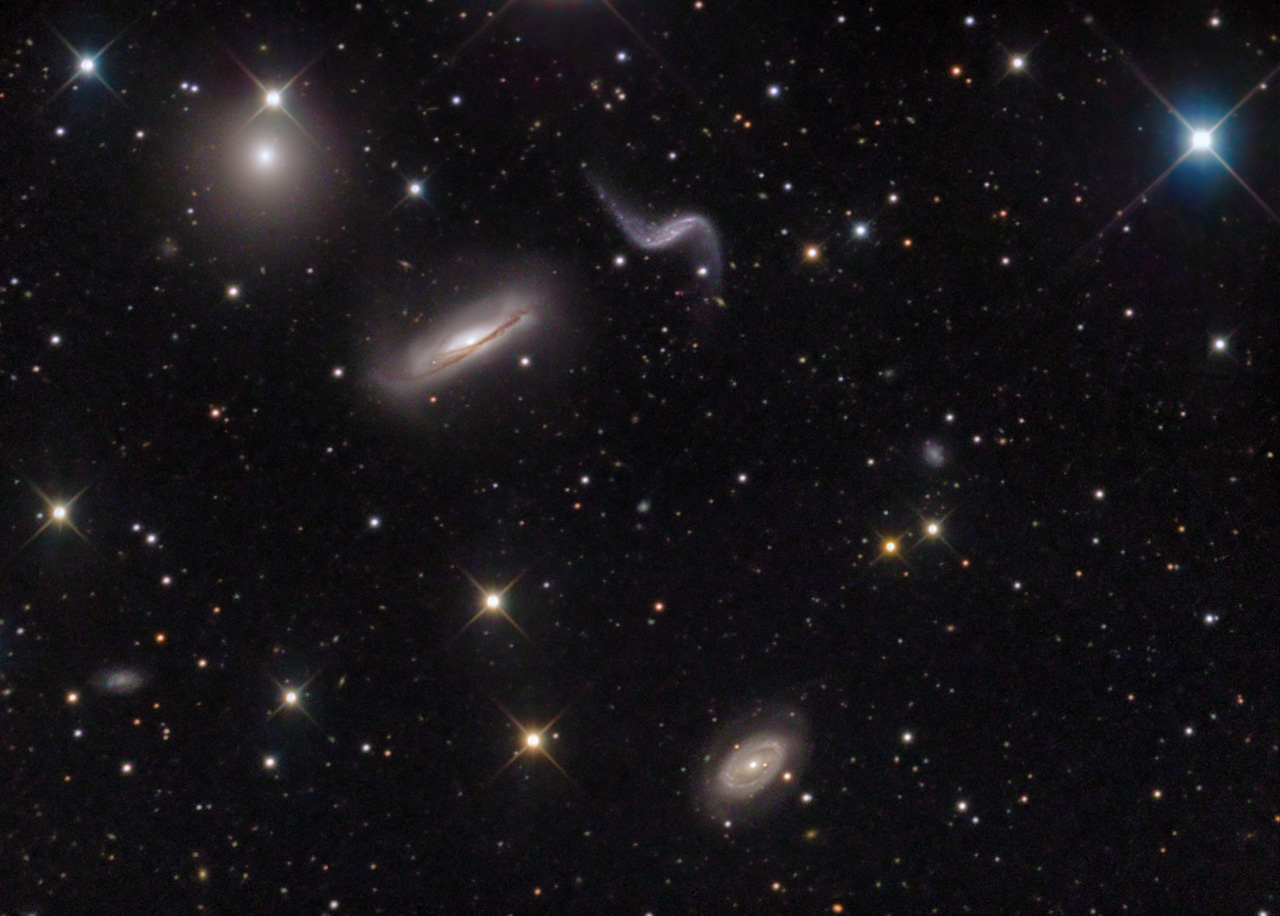
\includegraphics[width=\textwidth]{hickson44_masil_big.jpg}
                \newline
                {\tiny MASIL Imaging Team}
            \end{center}
        \end{column}
    \end{columns}
}


\frame
{
    \frametitle{Shear Measurement}

    \begin{itemize}

        \item Shear induces ellipticity

        \item Ellipticity is also altered by the atmosphere, the optics
            of the telescope, and the pixelization.
        
        \item These effects we call the Point Spread Function (PSF),
            must be modeled by studying stars.

        \item Surprisingly, the noise is the biggest problem:  All
            naive ellipticity measures are biased in the presence of
            noise.

    \end{itemize}
    \begin{center}
        \includegraphics[width=\textwidth]{great3-systematics.pdf}
        \newline
        {\tiny GREAT3 Team}
    \end{center}
}


\frame
{
    \frametitle{Ellipticity Measurement}

    \begin{itemize}

        \item Find the elliptical model that best fits the image

        \item In the presence of of noise, the best ellipticity yields a
            biased shear estimate: {\color{gold} $\sim 10$\%} for faint galaxies!
        \item Need to measure shear to {\color{gold} 0.1\%}.

    \end{itemize}
    \begin{center}

        % the trim values are the number of "big pixels" to trim off each side
        % or you can specify other units

        %\includegraphics[trim=left bottom right top, clip]{file}
        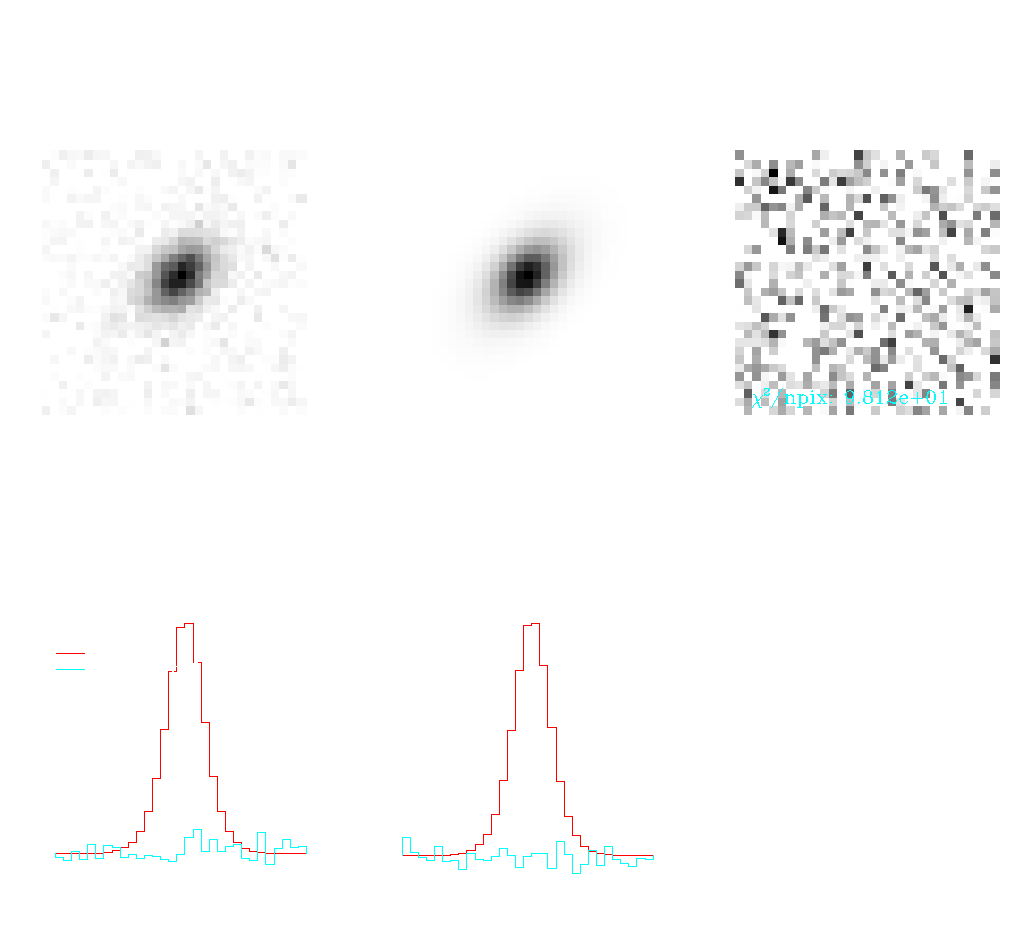
\includegraphics[trim=0 200 0 50,clip,width=0.8\textwidth]{example-fit-hi-s2n-invert.pdf}
    \end{center}
}



\frame
{
    \frametitle{Unbiased Shear Measurement}

    \setbeamerfont*{itemize/enumerate body}{size=\Large}
    \setbeamerfont*{itemize/enumerate subbody}{parent=itemize/enumerate body}
    \setbeamerfont*{itemize/enumerate subsubbody}{parent=itemize/enumerate body}
 
    \begin{itemize}

        \item In 2014 the first unbiased estimator was derived (Bernstein \&
            Armstrong, 2014):  theoretical only

            \begin{itemize}
                \item Using Bayesian principles: prior informatioin required from
                    low-noise data.

                \item Forget about individual galaxy, estimate shear of population
            \end{itemize}

        \item I developed an implementation for use on real images.


    \end{itemize}
}

\frame
{
    \frametitle{First Unbiased Shear Estimator}

    \begin{columns}

        \begin{column}{0.5\textwidth}    
            \begin{center}
                \hfill {\tiny Sheldon 2014}
                \newline
            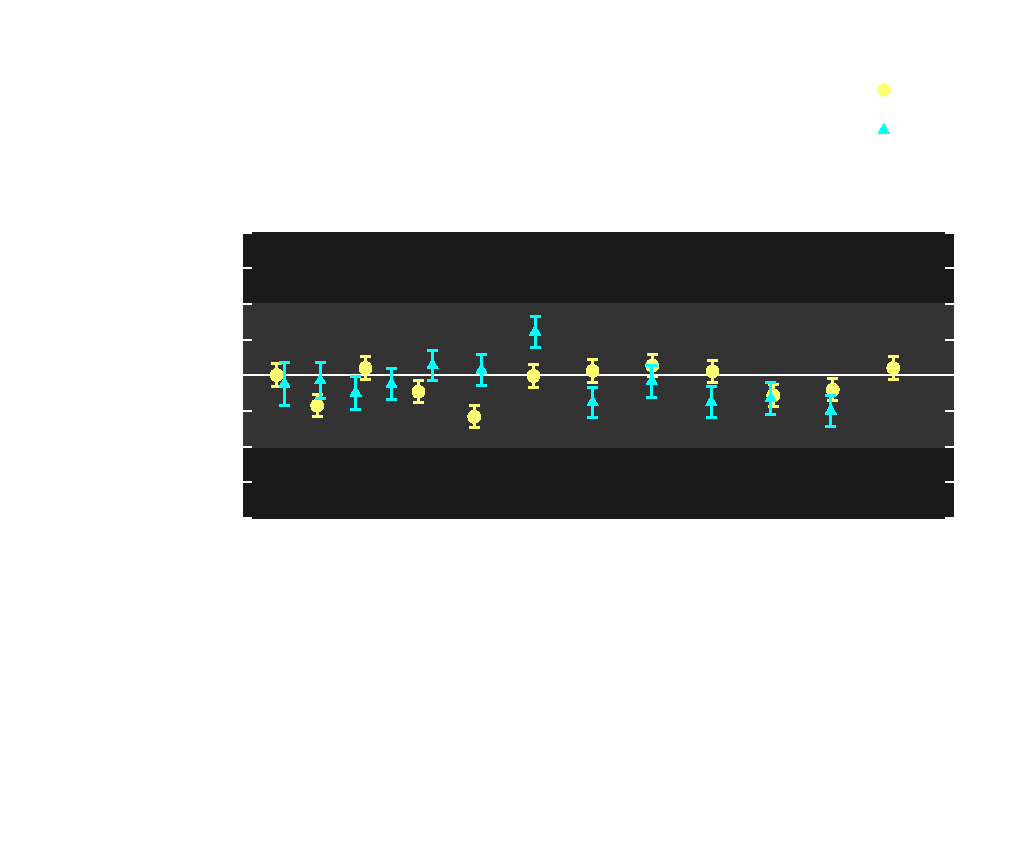
\includegraphics[width=\textwidth]{ngmix-flux-s2n-sigrat-20-invert.pdf}
            \end{center}
        \end{column}

        \begin{column}{0.5\textwidth}    
            \begin{itemize}

                \item Image simulations
                    \begin{itemize}
                        \item Galaxies
                        \item PSF
                        \item noise
                    \end{itemize}

                \item Tested shear recovery for different galaxy types
                    and noise levels

                \item Unbiased at the level required for current and future surveys.

                \item {\color{gold} Published (Sheldon 2014)}

            \end{itemize}
        \end{column}


    \end{columns}
}

\frame
{

    {\Huge Dark Matter Distribution in Galaxies and Clusters}

}



\frame
{
    \frametitle{Dark Matter Distribution}

    \setbeamerfont*{itemize/enumerate body}{size=\large}
    \setbeamerfont*{itemize/enumerate subbody}{parent=itemize/enumerate body}
    \setbeamerfont*{itemize/enumerate subsubbody}{parent=itemize/enumerate body}

    \begin{itemize}

        \item The program:
            \begin{enumerate}

                \item Identify lenses (galaxies or clusters)

                \item Identify background source galaxies.

                \item Measure the ellipticities of the source galaxies

                \item Average the ellipticities of background galaxies.

                \item Further average over many lenses

                \item Interpret in terms of the mean surface mass density {\color{gold}
                    $\Sigma$}

            \end{enumerate}
    \end{itemize}

    \begin{center}
        {\color{gold}
            {\huge
                $\overline{e}_{T}(R) \propto \overline{\Sigma}(<R) - \overline{\Sigma}(R)$
            }
        }
    \end{center}
}


\frame
{
    \frametitle{Sloan Digital Sky Survey}

    \begin{columns}
        \begin{column}{0.5\textwidth}    
            \begin{itemize}

                \item 2.5 Telescope at Apache Point New Mexico

                \item Imaged 10,000 sq. deg. in the northern sky through 5
                    filters, 126 Mpixel camera

                \item Imaging taken from 1999-2009

                \item Spectroscopy and redshifts for 1 million galaxies used
                    as {\color{gold} lenses }

                \item 50 million faint background galaxies used as {\color{gold} sources}
                    
            \end{itemize}
        \end{column}
        \begin{column}{0.5\textwidth}
            \begin{center}
                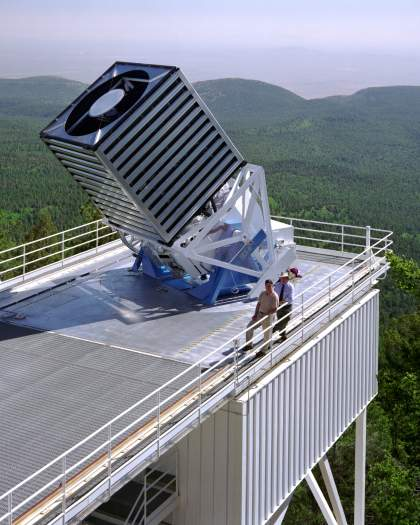
\includegraphics[width=\textwidth]{sdss-telescope.jpg}
                \newline
                {\tiny SDSS Telescope}
            \end{center}
        \end{column}
    \end{columns}
}

{
    \definecolor{mblack}{RGB}{0,0,0}
    \setbeamertemplate{background canvas}[vertical shading][bottom=black,top=black]

    \frame
    {	

        \begin{center}
            %\includegraphics[trim=left bottom right top, clip]{file}
            \includegraphics[trim=0 0 0 100,clip,width=0.85\textwidth]{M51-4x4.jpg}
            \newline
            \hfill {\tiny Whirlpool Galaxy, SDSS/Robert Lupton}
        \end{center}

    }
    \definecolor{mblack}{RGB}{50,50,50}
    \setbeamertemplate{background canvas}[vertical shading][bottom=mgray,top=mblack]
}

{
    \definecolor{mblack}{RGB}{0,0,0}
    \setbeamertemplate{background canvas}[vertical shading][bottom=black,top=black]


    \frame
    {
        \frametitle{Mass Distribution Around Galaxies}

        \begin{columns}
            \begin{column}{0.5\textwidth}    
                \begin{itemize}

                    \item Mean mass density in radial bins

                    \item Min radius 20 kpc max 10 Mpc {\color{gold} (1pc = 3.2ly)}

                    \item Light concentrated within 10 kpc

                    \item About 100 times more mass than in stars

                    \item On large scales looks like distribution of galaxies:
                        neighbors


                \end{itemize}
            \end{column}
            \begin{column}{0.5\textwidth}
                \begin{center}
                    %\includegraphics[trim=left bottom right top, clip]{file}
                    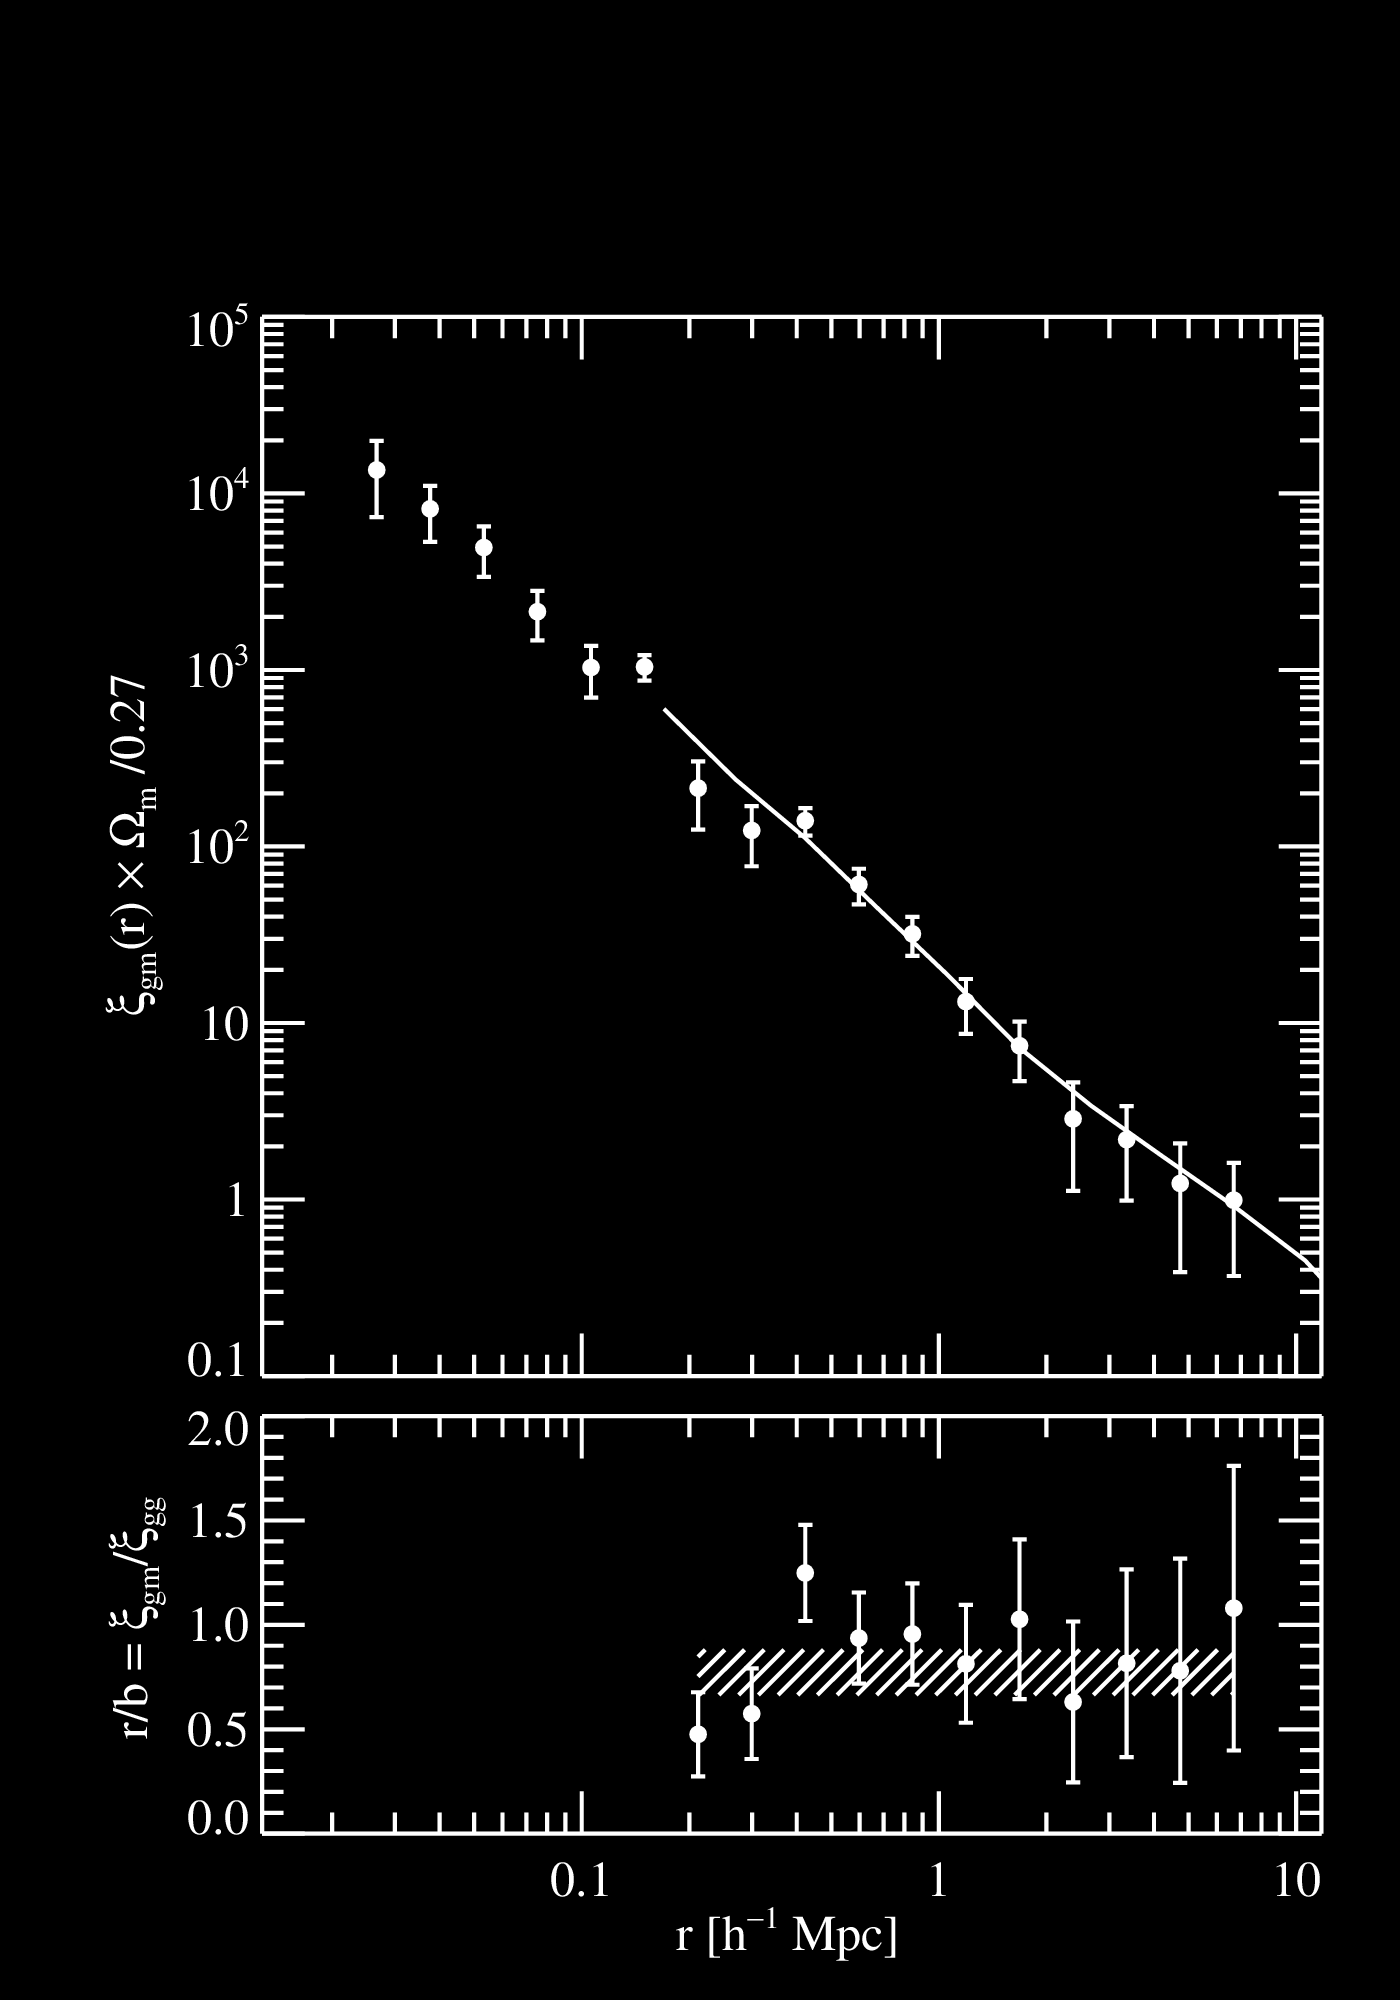
\includegraphics[trim=100 10 20 250,clip,width=\textwidth]{xi_all_idit_bias_icolor.png}
                    \newline
                    {\color{gold}Sheldon et al. 2004}
                \end{center}
            \end{column}
        \end{columns}
    }

    \definecolor{mblack}{RGB}{50,50,50}
    \setbeamertemplate{background canvas}[vertical shading][bottom=mgray,top=mblack]
}



\begin{comment}

    {
        \definecolor{mblack}{RGB}{0,0,0}
        \setbeamertemplate{background canvas}[vertical shading][bottom=black,top=black]


        \frame
        {
            \frametitle{Mass Distribution for Larger Galaxies}

                    \begin{center}
                        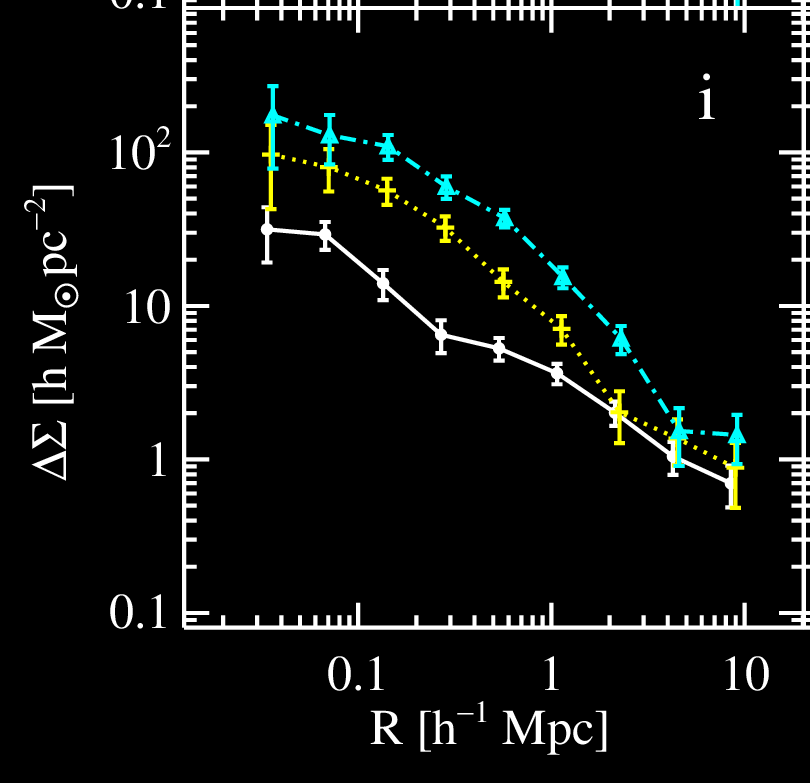
\includegraphics[trim=0 0 5 9,clip,width=0.8\textwidth]{deltasig_all_allband_bylum_icolor_crop.png}
                        \newline
                        {\color{gold}Sheldon et al. 2004}
                    \end{center}
        }

        \definecolor{mblack}{RGB}{50,50,50}
        \setbeamertemplate{background canvas}[vertical shading][bottom=mgray,top=mblack]
    }

    {
        \definecolor{mblack}{RGB}{0,0,0}
        \setbeamertemplate{background canvas}[vertical shading][bottom=black,top=black]



        \frame
        {
            \frametitle{As Predicted by CDM}

            \begin{itemize}

                \item Extended running power-law profile

                \item Shape of profile changes with size of galaxies

            \end{itemize}


            \begin{columns}
                \begin{column}{0.5\textwidth}    
                    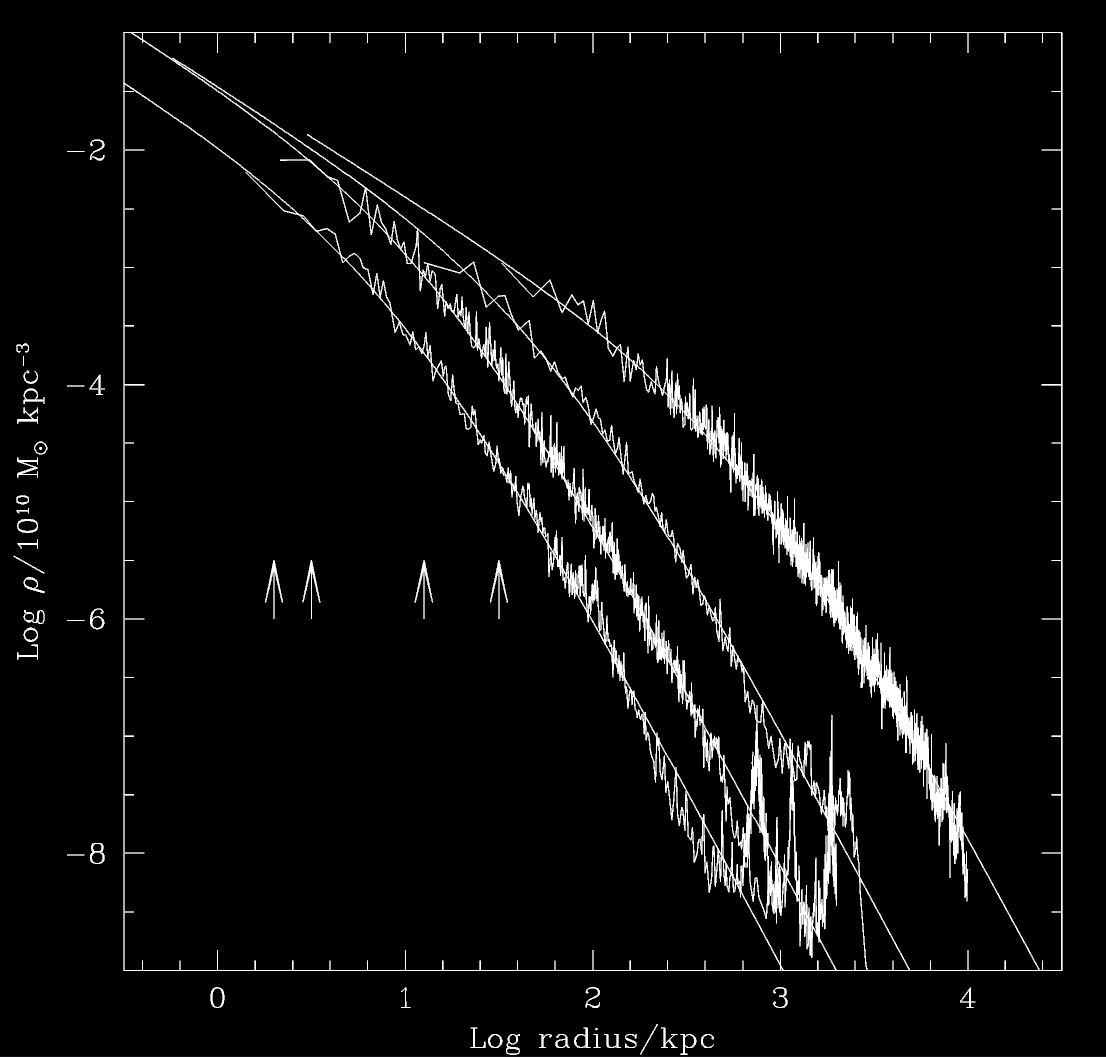
\includegraphics[width=\textwidth]{nfw.png}
                    \newline
                    {\tiny Navarro, Frenk, White 1996}
                \end{column}
                \begin{column}{0.5\textwidth}
                    %\includegraphics[trim=left bottom right top, clip]{file}
                    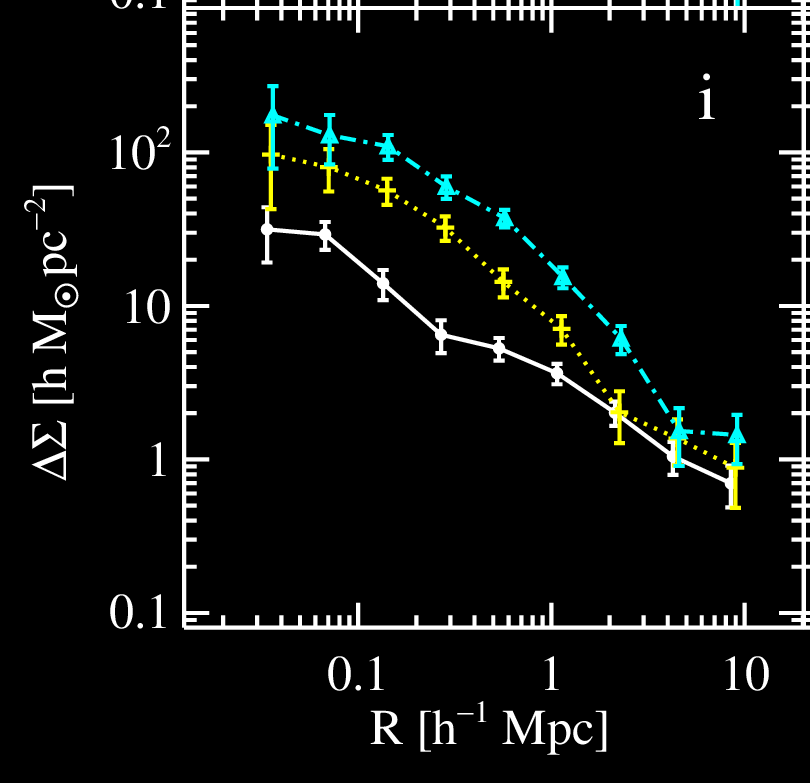
\includegraphics[trim=0 0 5 8,clip,width=\textwidth]{deltasig_all_allband_bylum_icolor_crop.png}
                    \newline
                    {\color{gold}Sheldon et al. 2004}
                \end{column}
            \end{columns}
        }

        \definecolor{mblack}{RGB}{50,50,50}
        \setbeamertemplate{background canvas}[vertical shading][bottom=mgray,top=mblack]
    }


\frame
{

    {\Huge Dark Matter Distribution in Clusters of Galaxies}

}

\end{comment}

{
    \definecolor{mblack}{RGB}{0,0,0}
    \setbeamertemplate{background canvas}[vertical shading][bottom=black,top=black]


    \frame
    {
        \frametitle{Galaxy Clusters}

        \begin{itemize}

            \item More useful than galaxies for learning about Dark Matter
            \begin{itemize}

                \item 100-1000 times more massive than galaxies: higher signal

                \item 10 times larger in extent: better resolution in radius to
                    study the mass profile

            \end{itemize}

        \end{itemize}
        \begin{center}
            %\includegraphics[trim=left bottom right top, clip]{file}
            \includegraphics[trim=0 300 0 500,clip,width=\textwidth]{abell1689_hubble_1280.jpg}
        \end{center}
            \hfill {\tiny NASA/ESA}
    }
    \definecolor{mblack}{RGB}{50,50,50}
    \setbeamertemplate{background canvas}[vertical shading][bottom=mgray,top=mblack]
}

{
    \definecolor{mblack}{RGB}{0,0,0}
    \setbeamertemplate{background canvas}[vertical shading][bottom=black,top=black]


    \frame
    {
        \frametitle{Mass Distriution in and around Galaxy Clusters}

        \begin{center}
            %\includegraphics[trim=left bottom right top, clip]{file}
            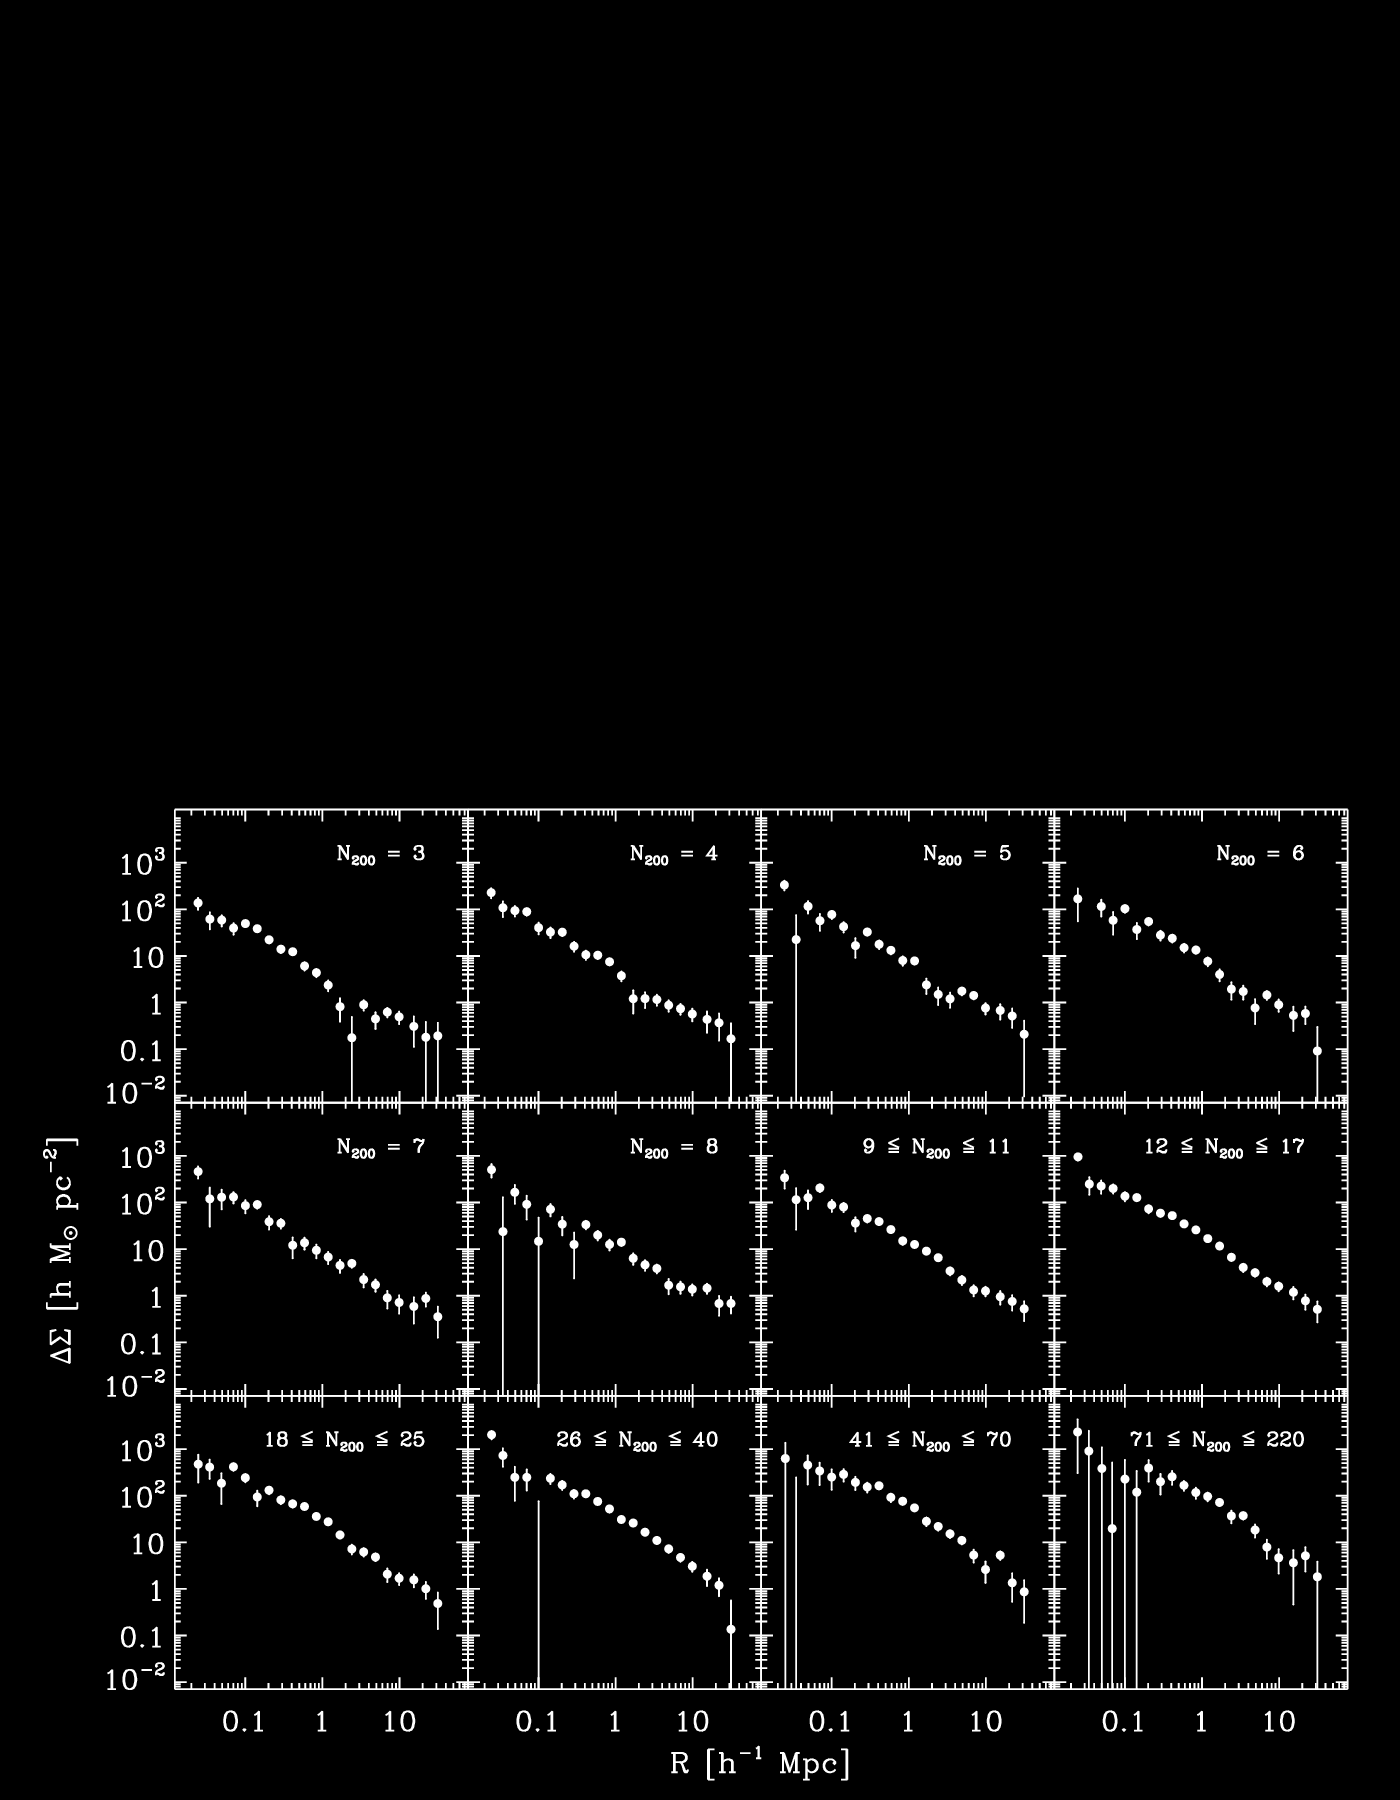
\includegraphics[trim=0 0 0 800,clip,width=0.9\textwidth]{maxbcg_sample21-22_ngals200_12_jackknife_icolor.png}
        \end{center}
        \hfill {\color{gold} Sheldon et al. 2009}
    }
    \definecolor{mblack}{RGB}{50,50,50}
    \setbeamertemplate{background canvas}[vertical shading][bottom=mgray,top=mblack]
}




{
    \definecolor{mblack}{RGB}{0,0,0}
    \setbeamertemplate{background canvas}[vertical shading][bottom=black,top=black]


    \frame
    {
        \frametitle{Interpretation in Terms of Universal Profile}

        \begin{center}
            %\includegraphics[trim=left bottom right top, clip]{file}
            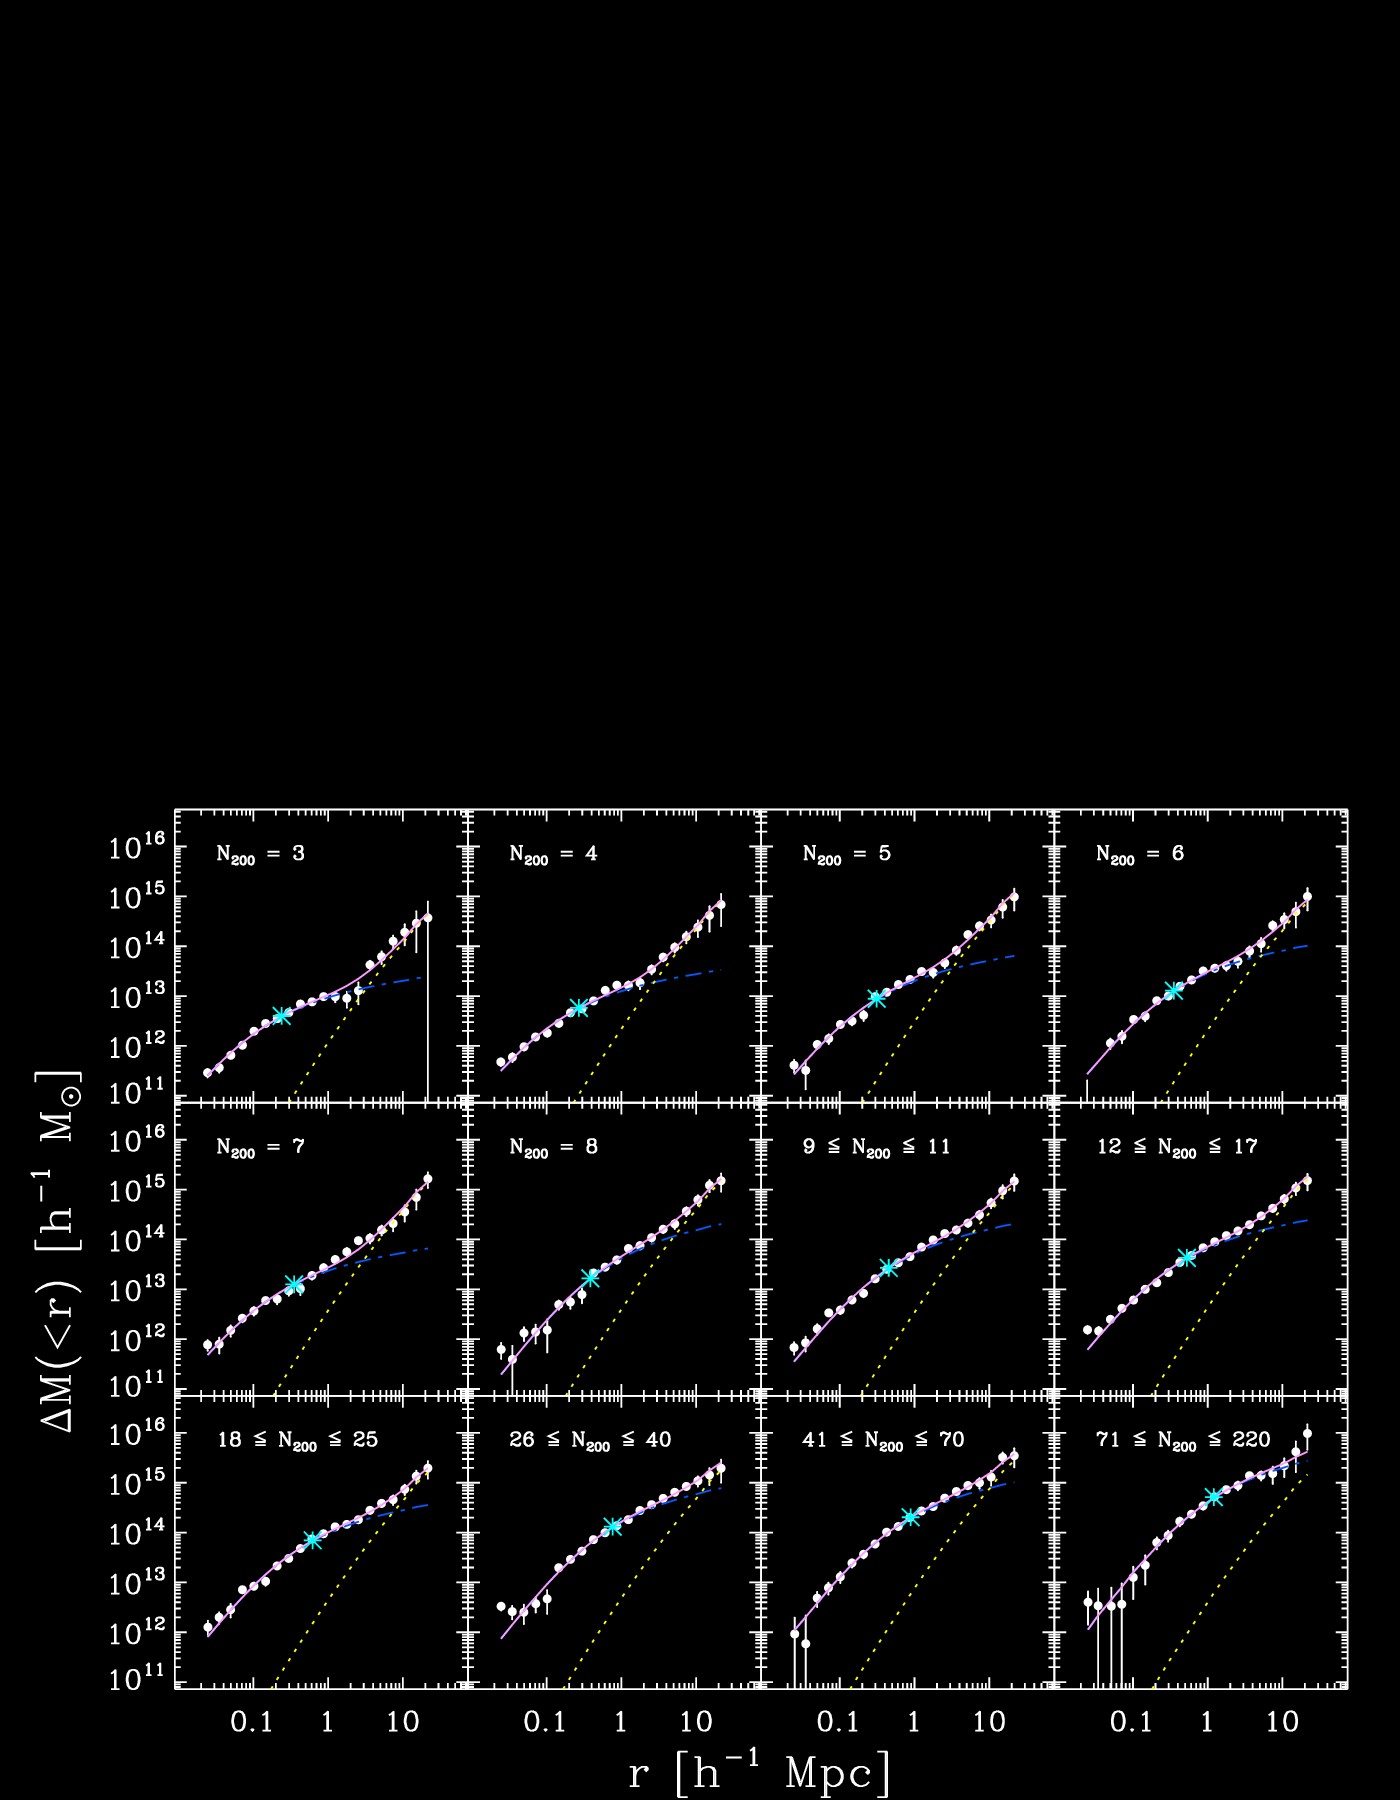
\includegraphics[trim=20 0 50 800,clip,width=0.9\textwidth]{m2l-ngals200_12-m21-22-l4-massfits-icolor.png}
        \end{center}
        \hfill {\color{gold} Sheldon et al. 2009}
    }

    \definecolor{mblack}{RGB}{50,50,50}
    \setbeamertemplate{background canvas}[vertical shading][bottom=mgray,top=mblack]
}

{
    \definecolor{mblack}{RGB}{0,0,0}
    \setbeamertemplate{background canvas}[vertical shading][bottom=black,top=black]


    \frame
    {
        \frametitle{Interpretation in Terms of Universal Profile}

        \begin{center}
            %\includegraphics[trim=left bottom right top, clip]{file}
            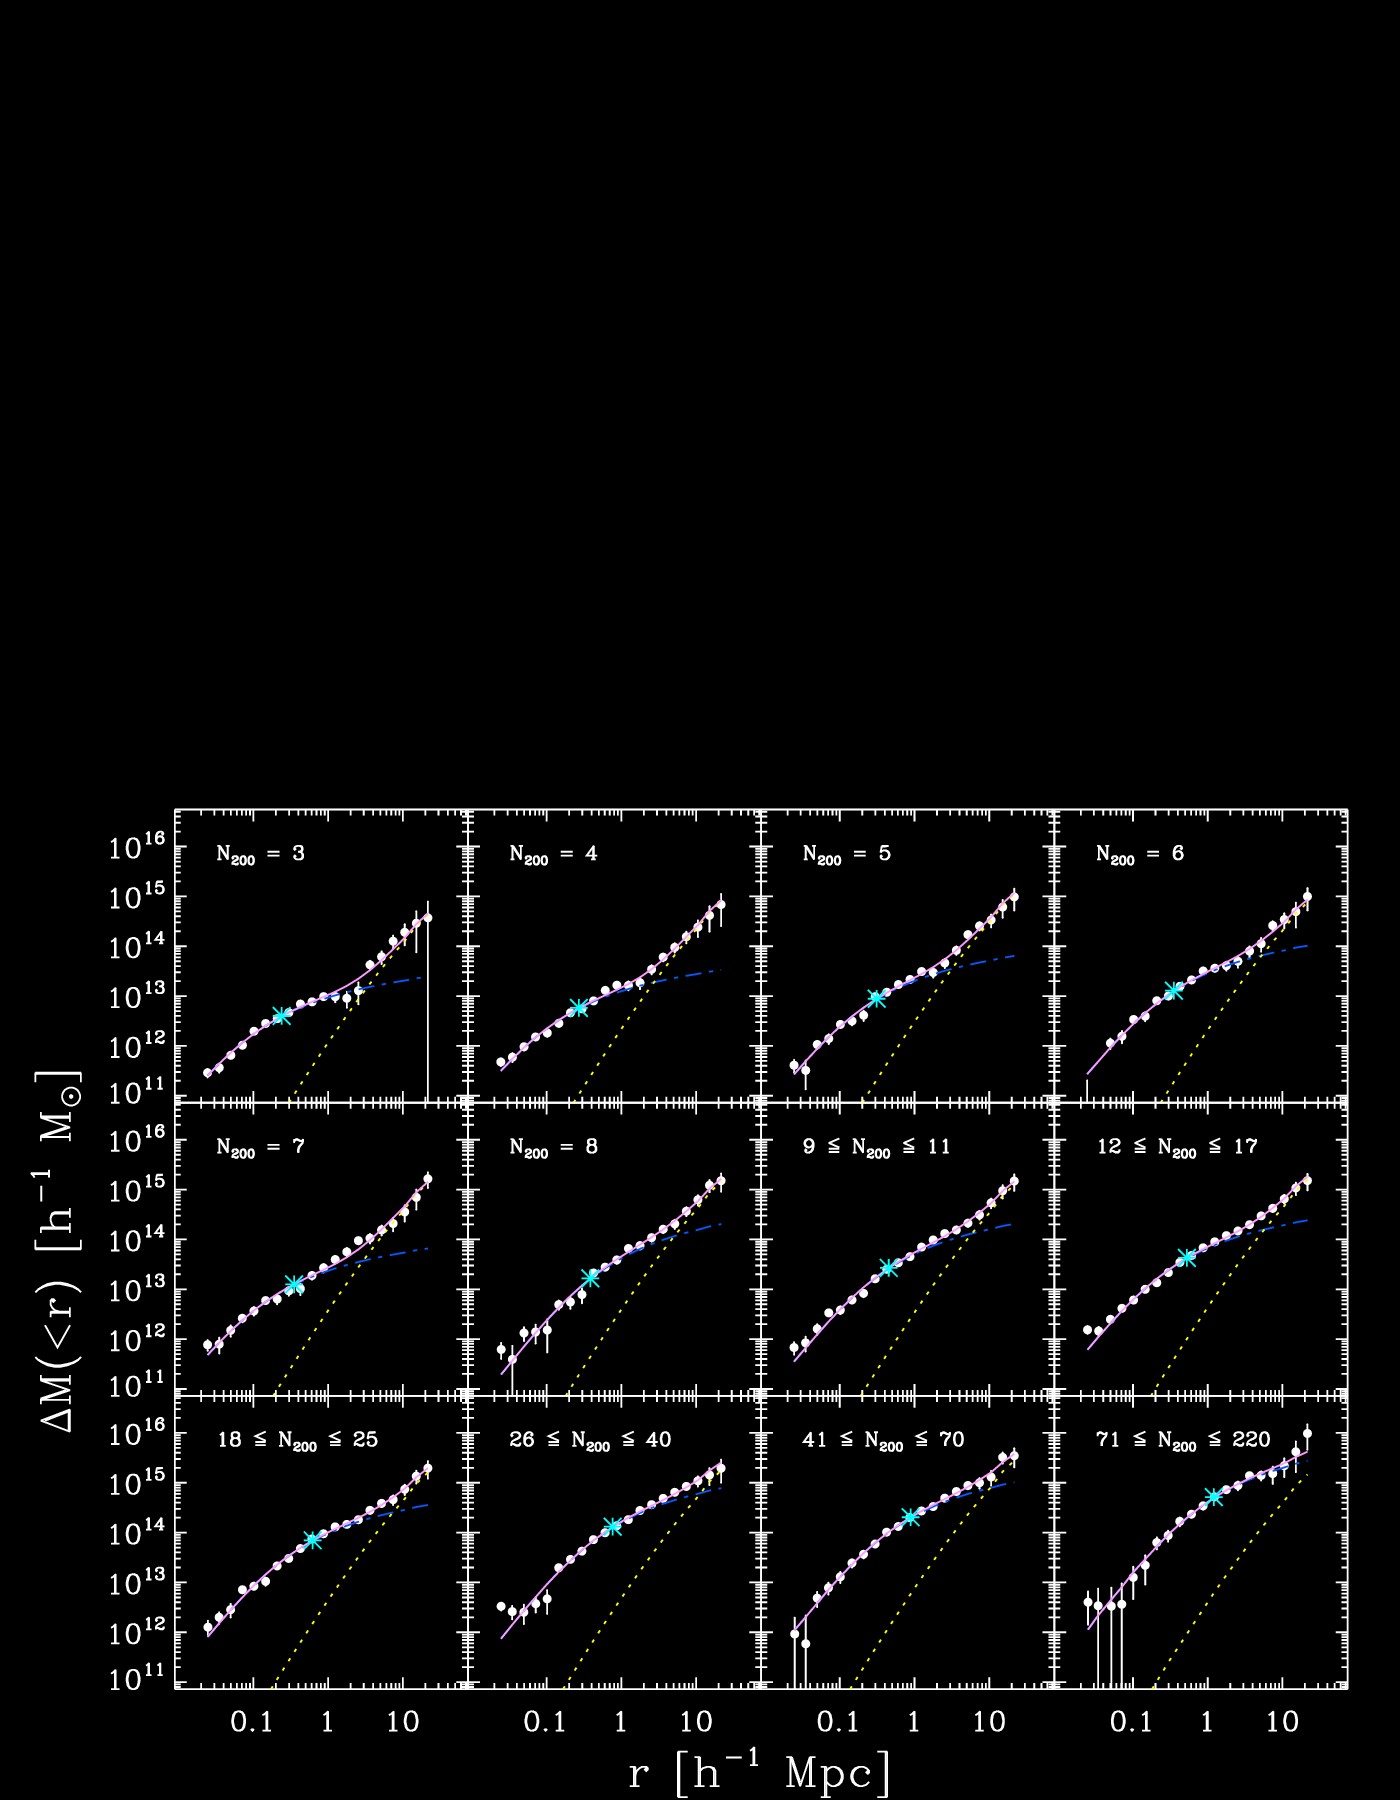
\includegraphics[trim=100 50 850 1390,clip,width=1\textwidth]{m2l-ngals200_12-m21-22-l4-massfits-icolor.png}
        \end{center}
        \hfill {\color{gold} Sheldon et al. 2009}
    }

    \definecolor{mblack}{RGB}{50,50,50}
    \setbeamertemplate{background canvas}[vertical shading][bottom=mgray,top=mblack]
}



\begin{comment}
    {
        \definecolor{mblack}{RGB}{0,0,0}
        \setbeamertemplate{background canvas}[vertical shading][bottom=black,top=black]


        \frame
        {
            \frametitle{Interpretation in Terms of Universal Profile}

            \begin{center}
                %\includegraphics[trim=left bottom right top, clip]{file}
                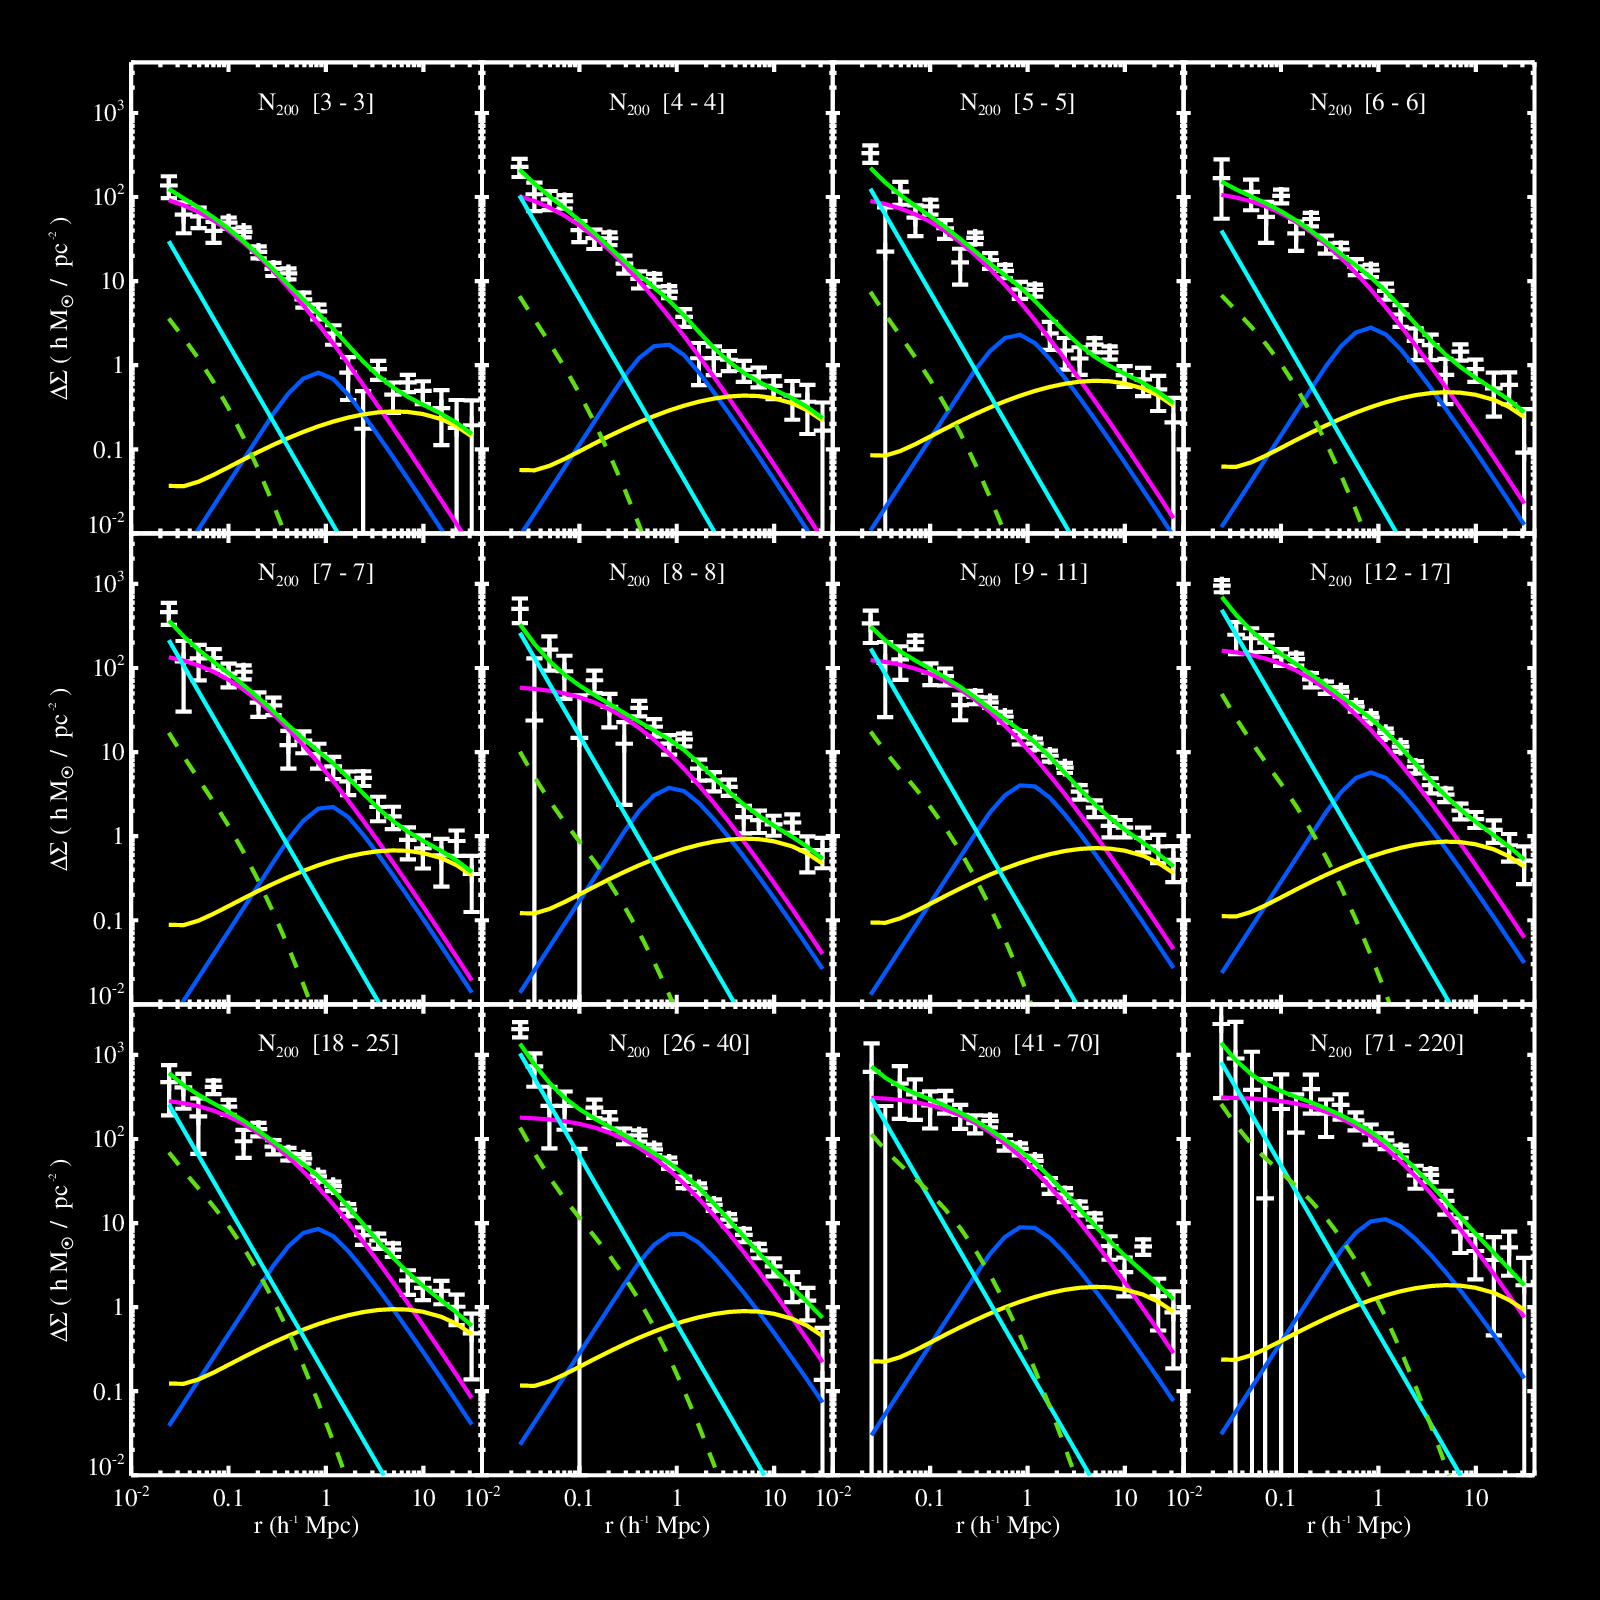
\includegraphics[trim=10 10 10 10,clip,width=0.7\textwidth]{Ngal200_DS_hfits_icolor.png}
            \end{center}
            \hfill {\color{gold} Johnston et al.}
        }

        \definecolor{mblack}{RGB}{50,50,50}
        \setbeamertemplate{background canvas}[vertical shading][bottom=mgray,top=mblack]
    }


    {
        \definecolor{mblack}{RGB}{0,0,0}
        \setbeamertemplate{background canvas}[vertical shading][bottom=black,top=black]


        \frame
        {
            \frametitle{Interpretation in Terms of Universal Profile}

            \begin{center}
                %\includegraphics[trim=left bottom right top, clip]{file}
                \includegraphics[trim=1050 450 50 480,clip,width=0.7\textwidth]{Ngal200_DS_hfits_icolor.png}
            \end{center}
            \hfill {\color{gold} Johnston et al.}
        }

        \definecolor{mblack}{RGB}{50,50,50}
        \setbeamertemplate{background canvas}[vertical shading][bottom=mgray,top=mblack]
    }

\end{comment}



{
    \definecolor{mblack}{RGB}{0,0,0}
    \setbeamertemplate{background canvas}[vertical shading][bottom=black,top=black]


    \frame
    {
        \frametitle{Mass-to-light Ratio: CDM Predicts Light Should be More Concentrated}

        \begin{center}
            %\includegraphics[trim=left bottom right top, clip]{file}
            \includegraphics[trim=0 0 0 800,clip,width=0.9\textwidth]{m2l-ngals200_12-m21-22-l4-m2lfits-color.png}
        \end{center}
        \hfill {\color{gold} Sheldon et al. 2009}
    }
    \definecolor{mblack}{RGB}{50,50,50}
    \setbeamertemplate{background canvas}[vertical shading][bottom=mgray,top=mblack]
}

{
    \definecolor{mblack}{RGB}{0,0,0}
    \setbeamertemplate{background canvas}[vertical shading][bottom=black,top=black]


    \frame
    {
        \frametitle{Mass-to-light Ratios and $\Omega_m$}

        \begin{columns}
            \begin{column}{0.6\textwidth}
                \begin{itemize}
                    \item $M/L$ reaches constant at large radius, same for all samples
                    \item Universal $M/L$

                    \item Multiply by the luminosity density in the universe to
                        get the universal mass density {\color{gold} $\rho_m = \bar{\ell} \times M/L$ }


                    \item Express as fraction of the universal energy density
                    %, independent of hubble parameter $H_0$

                    \item {\color{gold} $\Omega_m b_{M/L}^{-2} = 0.20 \pm 0.03$ }

                \end{itemize}
            \end{column}
            \begin{column}{0.4\textwidth}
                \centering
                %\includegraphics[trim=left bottom right top, clip]{file}
                \includegraphics[trim=0 0 930 800,clip,height=0.7\textheight]{m2l-ngals200_12-m21-22-l4-m2lfits-color.png}
                \newline
                {\color{gold}Sheldon et al. 2009}
            \end{column}
        \end{columns}
    }


    \definecolor{mblack}{RGB}{50,50,50}
    \setbeamertemplate{background canvas}[vertical shading][bottom=mgray,top=mblack]
}



{
    \definecolor{mblack}{RGB}{0,0,0}
    \setbeamertemplate{background canvas}[vertical shading][bottom=black,top=black]


    \frame
    {
        \frametitle{Total Mass in the Cluster}

        \begin{center}
            %\includegraphics[trim=left bottom right top, clip]{file}
            \includegraphics[width=0.7\textwidth]{mass-rich-plot-icolors.png}
            \newline
            \hfill {\color{gold} Johnston, Sheldon et al.}
        \end{center}
    }
    \definecolor{mblack}{RGB}{50,50,50}
    \setbeamertemplate{background canvas}[vertical shading][bottom=mgray,top=mblack]
}

\frame
{
    \frametitle{Cosmological Parameters}
    \begin{itemize}

        \item CDM also predicts $dN/dM$, the number of objects of a given mass, and
            this depends on {\color{gold} $\Omega_m$}.

            \begin{itemize}
                \item We know $dN/dn_{gals}$ and $M(n_{gals})$!

                \item Combine  $dN/dn_{gals}$ and $M(n_{gals})$ to get $dN/dM$ and infer
                    $\Omega_m$
                    (Rozo et al. 2010)

                    {\color{gold}
                        \begin{equation}
                            \Omega_m = 0.28 \pm 0.07 \nonumber
                        \end{equation}
                    }
            \end{itemize}

        \item Combine Mass/Number radial profiles with galaxy clustering 
            (Tinker et al. 2012)

            {\color{gold}
                \begin{equation}
                    \Omega_m = 0.29 \pm 0.03 \nonumber
                \end{equation}
            }


    \end{itemize}
}

\frame
{

    {\Huge Dark Energy }

}

{
    \definecolor{mblack}{RGB}{0,0,0}
    \setbeamertemplate{background canvas}[vertical shading][bottom=black,top=black]

    \frame
    {
        \frametitle{Dark Energy}

        %\fontsize{9}{0.8\baselineskip}
        \begin{columns}
            \begin{column}{0.4\textwidth}    
                \begin{itemize}

                    \item Astronomers tried to predict the brightness of a
                        standard candels at a known redshifts (type Ia
                        Supernovae)

                    \item They got the wrong answer assuming the universe is
                        homogeneous and filled with normal matter

                    \item Most easily explained if the universal expansion is accelerating.

                \end{itemize}
            \end{column}
            \begin{column}{0.6\textwidth}
                \begin{center}
                    \includegraphics[width=\textwidth]{riess-distmodulus.png}
                    \newline
                    {\tiny Riess et al. 2007}
                \end{center}
            \end{column}
        \end{columns}
    }

    \definecolor{mblack}{RGB}{50,50,50}
    \setbeamertemplate{background canvas}[vertical shading][bottom=mgray,top=mblack]
}



{
    \definecolor{mblack}{RGB}{0,0,0}
    \setbeamertemplate{background canvas}[vertical shading][bottom=black,top=black]


    \frame
    {
        The universe {\em is} homogeneous
        \begin{columns}[T]
            \begin{column}{0.55\textwidth}
                \includegraphics[trim=50 50 50 50,clip,width=\textwidth]{CMB-Tegmark.jpeg}
            \end{column}
            \begin{column}{0.55\textwidth}
                \vspace{10 mm}
                \includegraphics[width=\textwidth]{sdss-gals-blanton.jpg}
            \end{column}
        \end{columns}
        {\tiny \hfill WMAP (M. Tegmark), SDSS Galaxies (M. Blanton)}
    }
    \definecolor{mblack}{RGB}{50,50,50}
    \setbeamertemplate{background canvas}[vertical shading][bottom=mgray,top=mblack]

}




\frame
{
    \frametitle{Dark Energy Equation of State}

    \setbeamerfont*{itemize/enumerate body}{size=\Large}
    \setbeamerfont*{itemize/enumerate subbody}{parent=itemize/enumerate body}
    \setbeamerfont*{itemize/enumerate subsubbody}{parent=itemize/enumerate body}
 
    \begin{itemize}

        \item The universe seems to be accelerating

        \item The simplest approach is to add a term to Einstein's equations
        \begin{itemize}
            \item Cosmological Constant

            \item Or maybe exotic stuff.  Simplest model is uniform field with

                \vspace{5 mm}
                \begin{center}
                    {\color{gold}
                        {\huge $p = w \rho$}
                    }
                \end{center}
                \vspace{5 mm}

            \item Cosmological Constant has $w=-1$

            \item Current constraints $w \sim -1 \pm 0.1$

        \end{itemize}
    \end{itemize}

}


\frame
{
    \frametitle{Using Lensing to Measure Dark Energy}

    %\fontsize{9}{0.8\baselineskip}
    \begin{columns}
        \begin{column}{0.5\textwidth}    
            \begin{itemize}

                \item Lensing is geometrical, depends on the distances to all
                    components of the lens system

                \item Look at the dependence of the shear effect as a function
                    of the source redshift
                    
                \item Current lensing data does not probe a sufficent volume of
                    the universe

            \end{itemize}
        \end{column}
        \begin{column}{0.5\textwidth}
            \begin{center}
                \includegraphics[width=\textwidth]{scinv-example-invert.pdf}
            \end{center}
        \end{column}
    \end{columns}
}

\frame
{

    \frametitle{Dark Energy Survey (DES)}

    \fontsize{9}{0.8\baselineskip}

    \begin{columns}

        \begin{column}{0.4\textwidth}
            \includegraphics[scale=0.17]{ctio_blanco_crew_2013Oct-30-small-balance.jpg}
            \newline
            \hfill {\tiny Image: Brian Nord, FNAL}
        \end{column}


        \begin{column}{0.6\textwidth}

            \begin{itemize}

                \item Imaging survey of 5000 square degrees in the southern
                    sky in Chile.  5 optical filters

                \item New 500 Megapixel camera

                \item About 7 times the volume of SDSS: Study lensing as a
                    function of {\color{gold}cosmic time $\Rightarrow$ dark
                    energy}

                \item First light Fall 2012, survey start Aug. 31, 2013, end 2018.

                \item Study Dark Energy using weak lensing, galaxy clusters,
                    large scale structure and supernovae.

                \item Measure {\color{gold} $w$} to {\color{gold} $\pm 0.02$}

            \end{itemize}

        \end{column}

    \end{columns}

}

{
	\definecolor{mblack}{RGB}{0,0,0}
    \setbeamertemplate{background canvas}[vertical shading][bottom=black,top=black]
	
    \frame
    {

        \begin{center}
            %\includegraphics[width=1.1\textwidth]{ngc_new_v0-1398_20130130-mm1-2-950px.jpg}
            \includegraphics[width=1.1\textwidth]{DES-2013-01-medres.jpg}

            {\tiny \hfill NGC 1398, Erin Sheldon, Martin Murphy}
        \end{center}
    }

	\definecolor{mblack}{RGB}{50,50,50}
    \setbeamertemplate{background canvas}[vertical shading][bottom=mgray,top=mblack]

}

\frame
{

    \frametitle{DES at BNL}

    \setbeamerfont*{itemize/enumerate body}{size=\small}
    \setbeamerfont*{itemize/enumerate subbody}{parent=itemize/enumerate body}
    \setbeamerfont*{itemize/enumerate subsubbody}{parent=itemize/enumerate body}
 
    \begin{columns}
        \begin{column}{0.5\textwidth}    
            \begin{itemize}

                \item I've been working on DES since 2003

                \item I am a {\color{gold} builder} and {\color{gold} associate
                    member} with data rights for self, postdoc, students.

                \item Co-convener of weak lensing working group

                \item Responsible for one of the two shear measurement codes

                \item Leading the effort to measure lensing around galaxy clusters

                \item Andres Plazas BNL postdoc worked on detector
                    characterization and weak lensing of galaxy clusters

            \end{itemize}
        \end{column}
        \begin{column}{0.5\textwidth}
                \centering
                %\newline
                %\includegraphics[width=\textwidth]{ngc0894-rebin4.jpg}
                %\newline
                %\includegraphics[width=\textwidth]{decam-image-1-medres-crop.jpg}
                %\newline
                %{\tiny Camera Installation}
                \includegraphics[angle=90,origin=c,height=0.6\textheight,trim=0 0 200 0,clip]{ngc0894-rebin4.jpg}
                \newline
                {\tiny Image: Erin Sheldon}
        \end{column}
    \end{columns}

}

\frame
{

    \frametitle{\prelim\ Lensing Results from DES}

    %\setbeamerfont*{itemize/enumerate body}{size=\small}
    %\setbeamerfont*{itemize/enumerate subbody}{parent=itemize/enumerate body}
    %\setbeamerfont*{itemize/enumerate subsubbody}{parent=itemize/enumerate body}
 
    \begin{columns}
        \begin{column}{0.5\textwidth}    
            \begin{itemize}

                \item Results from science verification period

                \item {\color{gold} 3\% of final data }

                \item Mean lensing signal for 12,000 galaxy clusters found
                    using the RedMapper algorithm

            \end{itemize}
        \end{column}
        \begin{column}{0.5\textwidth}
            \begin{center}
                \includegraphics[width=\textwidth]{run-rm008-bin-zwide-jack-icolor.pdf}
                \newline
            \end{center}
        \end{column}
    \end{columns}

}

\begin{comment}
    \frame
    {

        \frametitle{Preliminary Lensing Results from DES}

        \begin{minipage}{\linewidth}
            \vspace{5mm}
            Binned by number of galaxies in the cluster
            \vspace{5mm}
        \end{minipage}

        \begin{minipage}{\linewidth}
            \centering
            \includegraphics[width=0.8\textwidth]{run-rm008-bin-lbin12-zwide-jack-icolor.pdf}
        \end{minipage}

    }
\end{comment}

\frame
{

    \frametitle{Lensing as a Function of Cosmic Time}
 
    \begin{minipage}{\linewidth}
        \vspace{5mm}
        Binned by redshift, or cosmic time.  {\color{gold} Not possible with SDSS }
        \vspace{5mm}
    \end{minipage}
    \begin{minipage}{\linewidth}
        \centering
        \includegraphics[width=0.6\textwidth]{run-rm008-bin-lgt05-zbin4-jack-icolor.pdf}
    \end{minipage}

}

\frame
{
    \frametitle{DES: Future Work}

    \setbeamerfont*{itemize/enumerate body}{size=\Large}
    \setbeamerfont*{itemize/enumerate subbody}{parent=itemize/enumerate body}
    \setbeamerfont*{itemize/enumerate subsubbody}{parent=itemize/enumerate body}
 
    \begin{itemize}

        \item Process more data!

        \item The codes are vetted, good enough for studies on early data

        \item Look in detail at the dark matter profiles: Do they evolve over
            time as predicted by CDM?

        \item Cosmological analysis requires more data.  Approximately 2 years
            timescale.

    \end{itemize}

}


\frame
{
    \frametitle{The Long View: LSST}

    %\setbeamerfont*{itemize/enumerate body}{size=\Large}
    %\setbeamerfont*{itemize/enumerate subbody}{parent=itemize/enumerate body}
    %\setbeamerfont*{itemize/enumerate subsubbody}{parent=itemize/enumerate body}
    \begin{columns}

        \begin{column}{0.5\textwidth}    
            \includegraphics[width=\textwidth]{Telescope_Side_2-140-scaled.jpg}
            \newline
            \includegraphics[width=\textwidth]{LSST_Rendering_VK_scaled.jpg}
        \end{column}

        \begin{column}{0.5\textwidth}    

            \begin{itemize}

                \item Large Synoptic Survey Telescope (LSST)

                \item New 3.2 Megapixel camera, the world's largest

                \item New 8.4 Meter telescope

                \item Survey half the sky; 1000 visits per field over 10 years, each
                    with depth of DES 

                \item Entering construction phase; First light 2020

            \end{itemize}
        \end{column}


    \end{columns}
}

\frame
{
    \frametitle{LSST}

    %\setbeamerfont*{itemize/enumerate body}{size=\Large}
    %\setbeamerfont*{itemize/enumerate subbody}{parent=itemize/enumerate body}
    %\setbeamerfont*{itemize/enumerate subsubbody}{parent=itemize/enumerate body}
    %\begin{columns}
    %    \begin{column}{0.5\textwidth}    

            \begin{itemize}

                \item BNL has been involved since 2004

                \item BNL Instrumentation responsible for CCDs, electronics
                    and rafts.


            \end{itemize}
    %    \end{column}
    %    \begin{column}{0.5\textwidth}    
            \centerline{\includegraphics[width=0.7\textwidth]{lsst-folks.jpg}}
            %\newline
            \hfill {\tiny Some BNL LSST Folks}
    %    \end{column}
    %\end{columns}
}

\frame
{
    \frametitle{LSST}

    %\setbeamerfont*{itemize/enumerate body}{size=\Large}
    %\setbeamerfont*{itemize/enumerate subbody}{parent=itemize/enumerate body}
    %\setbeamerfont*{itemize/enumerate subsubbody}{parent=itemize/enumerate body}
    \begin{columns}
        \begin{column}{0.5\textwidth}    

            \begin{itemize}

                \item I am transitioning to LSST from DES work, full time by
                    2019

                \item I am incorporating my shear code into the LSST framework
                    now. 

                \item Raw shear sensitivity of LSST is $\sim$ 5 times that of
                    DES, {\color{gold} with more leverage over cosmic time}

                \item Constrain  {\color{gold} $w$} to the sub-percent level.

                \item Study time dependence of dark energy properties: is {\color{gold} $w$ } constant?

            \end{itemize}
        \end{column}
        \begin{column}{0.5\textwidth}    
            \includegraphics[width=\textwidth]{mirror-casting-banner.jpg}
            \newline
            \vspace{2mm}
            \includegraphics[width=\textwidth]{Group_photo-half-scaled.jpg}
            \newline
            \hfill {\tiny Image: LSST Collaboration}
        \end{column}
    \end{columns}
}


%\includegraphics[width=\paperwidth,height=\paperheight]{ngc_new_v0-1398_20130130-mm1-2-950px.jpg}}
\usebackgroundtemplate{%
\includegraphics[height=\paperheight]{DES-2013-01-medres.jpg}}
\frame
{

    {\Huge Summary}

    \begin{columns}
        \begin{column}{0.65\textwidth}
            \begin{itemize}
                    {\color{white}

                        %\item Weak lensing is our best method to study the
                        %    distribution of Dark Matter in the universe

                        \item Predictions of Cold Dark Matter theory confirmed
                            \begin{itemize} 

                                \item The distribution of mass in galaxies and
                                    clusters follows a ``universal profile''
                                    
                                \item Universal profile is a running power law, no
                                    exponential cutoff like the light

                                \item Dark Matter is distributed smoothly throughout
                                    the universe, not bound in compact clumps like the
                                    disspiative baryonic material
                            \end{itemize}

                        \item With DES, lensing will mature as a probe of Dark Energy

                        \item This work will culminate in LSST

                    }
            \end{itemize}
        \end{column}
        \begin{column}{0.35\textwidth}
        \end{column}
    \end{columns}
}



\end{document}
